% Using a4paper and 12pt font by default
\documentclass[12pt, a4paper]{article}

\usepackage[polish, british]{babel}

% Bibliography
\usepackage[backend=biber, giveninits=true, natbib=true, style=numeric, sorting=nty]{biblatex}
\addbibresource{references.bib}

\DeclareNameAlias{sortname}{family-given}
\DeclareNameAlias{default}{family-given}

% Use more than one optional parameter in a new commands
\usepackage{xargs}

% Colored text etc.
\usepackage[pdftex,dvipsnames]{xcolor}

% Quotation marks
\usepackage[utf8]{inputenc}

% Pictures and /includegraphics
\usepackage{graphicx}
\usepackage{wrapfig}
\usepackage{float}

% Links in the table of contents + other stuff
\usepackage[hidelinks, linktoc=all]{hyperref}

% Support multi-page code listings
\usepackage[all]{hypcap}
\usepackage{subcaption}

% Times New Roman font
\usepackage[T1]{fontenc}
\usepackage{newtxmath,newtxtext}

% Margins
\usepackage[margin=2.5cm]{geometry}

% Interline
\usepackage{setspace}
\setstretch{1.5}

% Footnotes
\usepackage[bottom]{footmisc}

% Captions
\usepackage{caption}

% To-do notes
\usepackage[colorinlistoftodos,prependcaption,textsize=tiny]{todonotes}
\newcommandx{\unsure}[2][1=]{\todo[linecolor=red,backgroundcolor=red!25,bordercolor=red,#1]{#2}}
\newcommandx{\change}[2][1=]{\todo[linecolor=blue,backgroundcolor=blue!25,bordercolor=blue,#1]{#2}}
\newcommandx{\info}[2][1=]{\todo[linecolor=OliveGreen,backgroundcolor=OliveGreen!25,bordercolor=OliveGreen,#1]{#2}}
\newcommandx{\improvement}[2][1=]{\todo[linecolor=Plum,backgroundcolor=Plum!25,bordercolor=Plum,#1]{#2}}

% Code highlighting
\usepackage{minted}
\usemintedstyle{tango}

% New line after paragraph title
\newcommandx{\myparagraph}[1]{\paragraph{#1}\mbox{}}

% List stuff easily
\usepackage{multicol}
\usepackage[sharp]{easylist}

\let\OldEasylist\easylist
\let\OldEndEasylist\endeasylist
\renewenvironment{easylist}{%
    \OldEasylist%
    \ListProperties(Progressive*=3ex, Start1=1)%
}{%
    \OldEndEasylist%
}%

% Listing & picture counter
\usepackage{chngcntr}
\counterwithin{listing}{section}
\counterwithin{figure}{section}
\counterwithin{table}{section}

% Unbold the subsubsection and paragraph
\usepackage{titlesec}

\titleformat*{\subsubsection}{\normalfont\fontsize{13pt}{13pt}\selectfont}
\titleformat*{\paragraph}{\normalfont\itshape}

% Paragraph numbers
% \setcounter{secnumdepth}{4}


% Double abstract
\newenvironment{abstractpage}
  {\cleardoublepage\vspace*{\fill}\thispagestyle{empty}}
  {\vfill\cleardoublepage}
\renewenvironment{abstract}[1]
  {\bigskip\selectlanguage{#1}%
   \begin{center}\bfseries\abstractname\end{center}}
  {\par\bigskip}

% Title page
\usepackage{pdfpages}

% Hyphenation rules, etc.
\usepackage{csquotes}

\begin{document}

% Title page
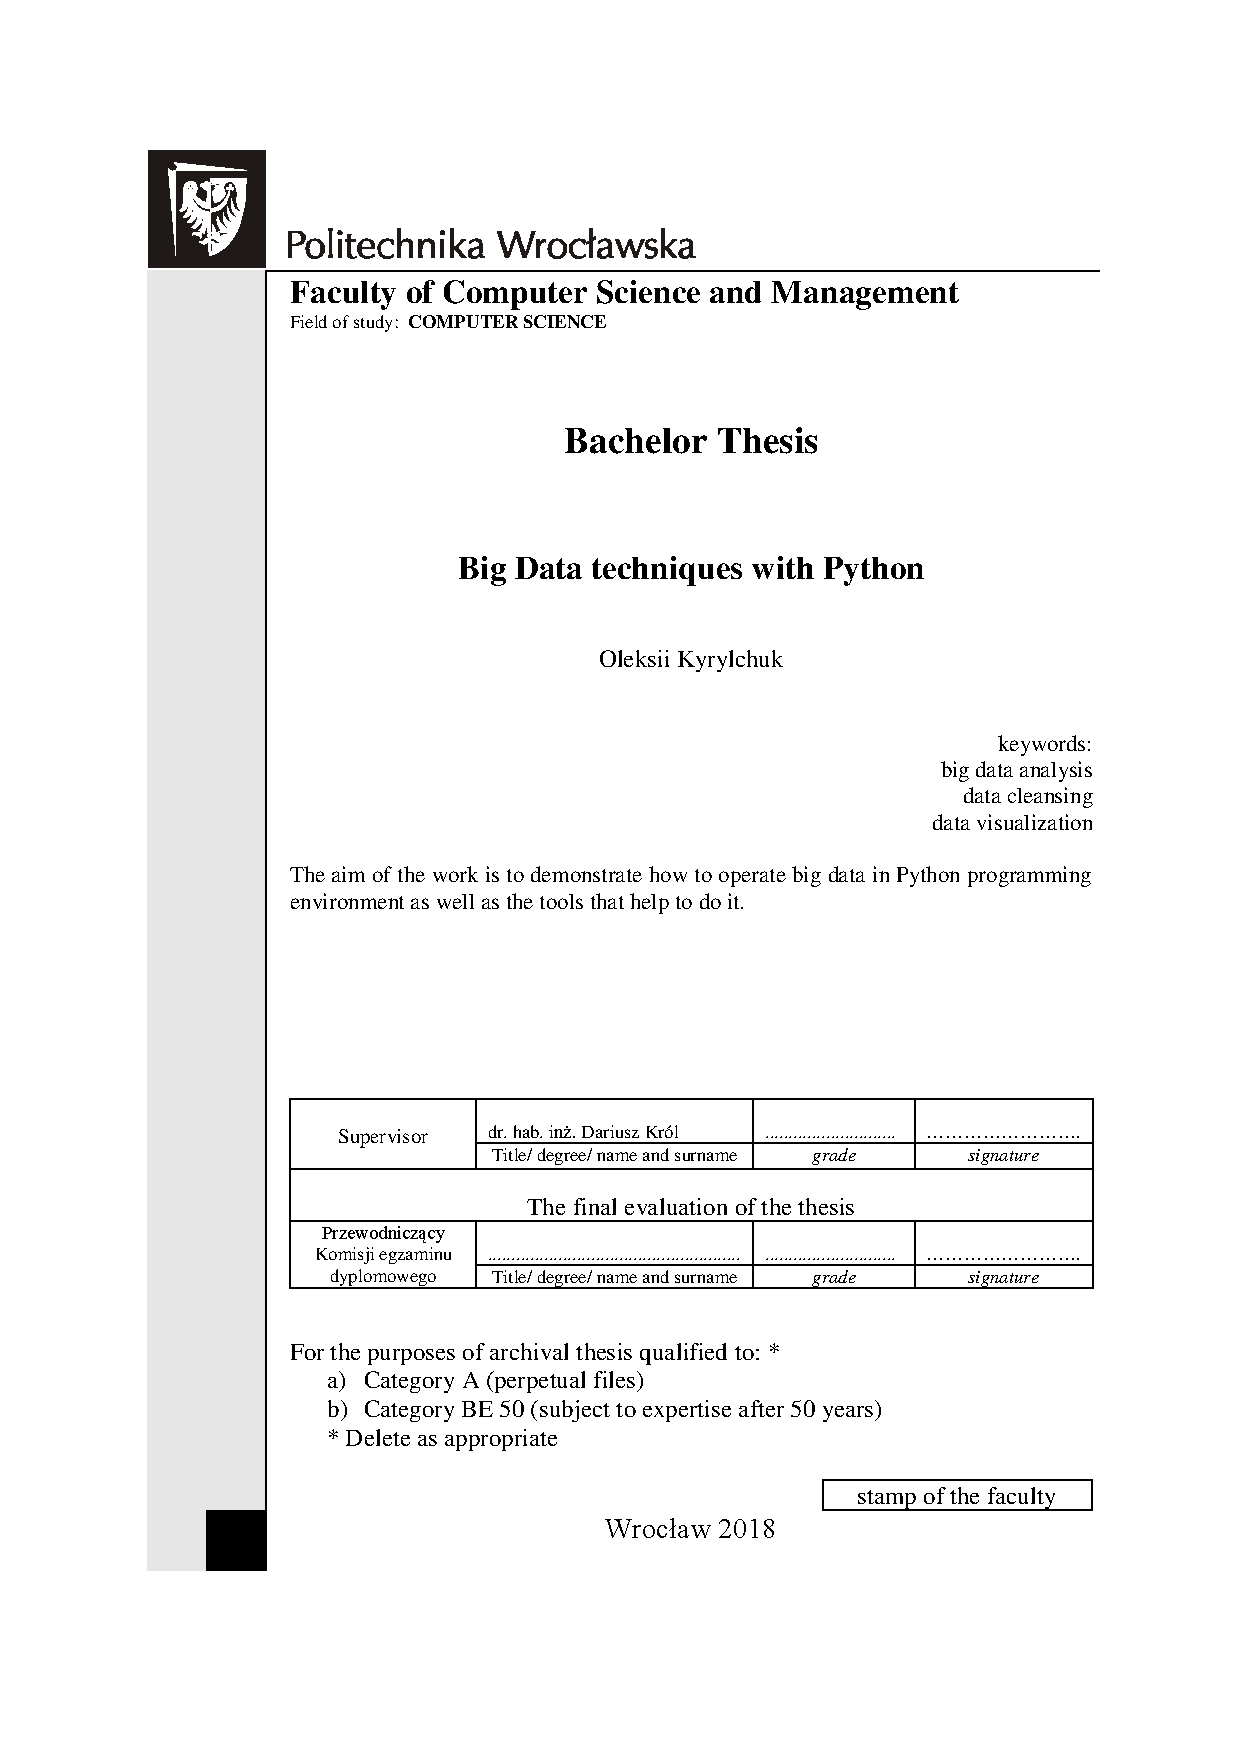
\includepdf[pages={1}]{title_page.pdf}

% Special page
\vspace*{\fill}
\begin{center}
The writing of the thesis has been requested.
\end{center}
\vspace{\fill}
\newpage

% Table of Contents
\tableofcontents
\newpage

% Misc - todelete
\listoftodos[Temporary Notes]
\newpage
% Abstract

\begin{abstractpage}
\begin{abstract}{polish}
    blablabla
\end{abstract}

\begin{abstract}{british}
    blablabla
\end{abstract}
\end{abstractpage}




%===============================================================================
\newpage
\section{INTRODUCTION}
%===============================================================================

%-------------------------------------------------------------------------------
\subsection{State of the Art in Data Science}
%-------------------------------------------------------------------------------
\improvement[inline]{Use stuff from the presentation}
\begin{easylist}
# Why is data analysis useful?
## Modern amounts of data explanation
## Data analysis explanation
# What tools are used to deal with large amounts of data?
## Traditional - ETL and DW (microsoft, qlikview, ...)
## Explorational - spark, R, python, matlab
# Why choose python?
## Advantages and disadvantages of using python
## Overview of chosen packages
\end{easylist}

\change[inline]{Rewrite everything}
%-------------------------------------------------------------------------------
\subsection{Goals of the Research}
%-------------------------------------------------------------------------------
In the modern world, big data and machine learning are becoming more and more prominent as companies such as Facebook, Google and Amazon gather and analyze all sorts of data from their users. But which tools are they using to do it?

Right now, the two main languages in data science are \mintinline{python}{Python} and \mintinline{python}{R}, while \mintinline{python}{Matlab} is also quite popular despite only being used in the academic environment.

This work's objective is to show how to use the Python 3 programming language in dealing with different kinds of data, and to help clarify any problems that might come up. It may be useful for long-term users of other languages that want to try Python out as well as users of Python 2, support for which will be stopped in 2020.
%-------------------------------------------------------------------------------
\subsection{Thesis Overview}
%-------------------------------------------------------------------------------
This work will be split into three parts, each working with a different dataset.

In the first part, I'll show you how to obtain, plot and predict stocks based on the last 17 years' worth of stock data from NYSE\footnotemark. I'll also cover some common problems that might occur when one is trying to deal with such amount of data.
\footnotetext{New York Stock Exchange}

In the second part, I'll cover scraping facebook's API, and plotting geolocation data of their events. I'll also discuss some problems that might occur while trying to download data, as well as how to use latest tools from Python (like the asyncio library) to speed up the data gathering part greatly. I'll also give you a brief overview of the current data visualization landscape, and show you which plotting packages are the best to use when dealing with geolocation data.

In the third part, I'll delve into the YouTube system, and will try to download and analyze their videos.

Lastly, the fourth part will contain conclusions.

%===============================================================================
\newpage
\section{TIME SERIES DATA ANALYSIS}
%===============================================================================
%-------------------------------------------------------------------------------
\subsection{Project Overview}
%-------------------------------------------------------------------------------

\subsubsection{Goals}

\begin{itemize}
	\item To show how to use python to obtain stock price data
	\item To show how to visualize the aforementioned data in different ways
	\item To show how to predict future prices by using a LSTM neural network
\end{itemize}

\subsubsection{Description}

This project will focus on dealing with time series data, which will be represented by the stock price data. It will contain four sections.

In the first one, I will show how to use the pandas-datareader package to download stocks traded on the New York Stock Exchange (NYSE) from the yahoo! finance website and merge them into one comma separated file.

In the second section, I will cover simple visualizations of singular stocks using the matplotlib package, which will include moving average and candlestick plots.

In the third section, I will cover visualization of a stock correlation matrix, which will, as opposed to the simple plots, include all of the stocks that were downloaded and not only one of them.

In the fourth and final section, I will demonstrate how to make a LSTM neural network for predicting the stock prices using the keras package and how to plot the predictions it generates, as well as cover how to use the pickle package to serialize python objects.


%-------------------------------------------------------------------------------
\newpage
\subsection{Data gathering (pandas-datareader)}
%-------------------------------------------------------------------------------

\myparagraph{Goal}

The goal of this section is to show how to use python to obtain stock price data, and transform it for further use.

\myparagraph{Process description}

\begin{figure}[H]
    \centering
    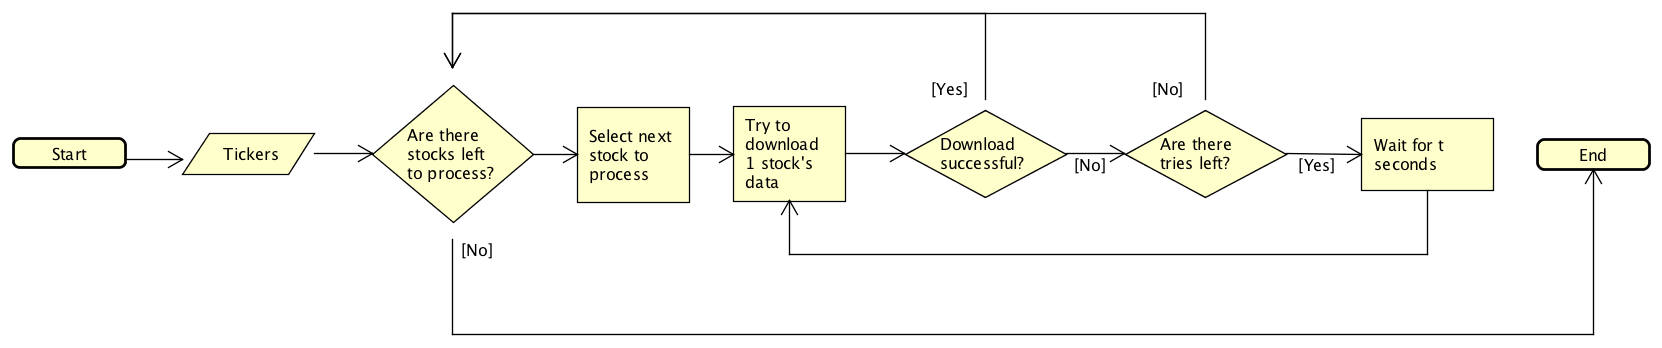
\includegraphics[width=\textwidth]{src/stocks/etl/stocks_download_chart}
    \caption{Stocks download flowchart}
    \label{fig:stocks_download_chart}
\end{figure}

As you can see on the figure \ref{fig:stocks_download_chart}, the download process can only begins after you have specified the tickers, or short names of the companies that you want to download the data for.

There are a couple of methods to obtain a list of tickers that you want to analyze: you could go through the companies that interest you and look up the ticker for every one of them, you could use a package called BeautifulSoup to obtain the tickers by scraping a webpage, or, if you are dealing with all of the stocks traded on a particular market (like we are here with NYSE), the official webpage for that market usually provides such a list. In this case, I have downloaded a list of all tickers from NYSE from the official NASDAQ website \cite{nasdaq_companylist} and saved the ticker column from the provided file  manually.

It is possible to just go trough them one by one and call the download function for every ticker, but that approach may be detrimental due to the fact that sometimes yahoo finance’s API  just outright refuses the pandas-datareader’s connection attempts, probably due to a large number of requests from one IP address.

Due to this inconsistency, we have to incorporate some fail-saves into the code, like checking whether the download was completed successfully and repeating it if something went wrong. The timeout between tries is also introduced here to avoid stressing the yahoo servers too much, and to avoid being flagged as a malicious user.

After a stock is processed this way, we save the data if we have successfully downloaded it, and go to the next stock in the list. While this approach doesn’t guarantee that 100\% of the stocks will get downloaded, it protects us from being stuck in an infinite loop due to yahoo finance not having a data for a certain stock.

\myparagraph{Used packages}

Below you will find packages that will be used in this section of the project.

\bgroup
  \inputminted[linenos, breaklines=true, fontsize=\scriptsize, firstnumber=last]{python}{src/stocks/etl/0a_imports.py}
  \captionof{listing}{Imports}
  \label{listing:setl_0a_imports}
\egroup


\myparagraph{Tqdm}

Please pay attention to the use of the tqdm package in the listing \ref{listing:setl_1_download}. It is a very useful package that allows you to create progress bars that work in both console and jupyter notebooks, and help with determining how much time is left in a long process, or how many things we have already processed. To use it, you can just change \texttt{for i in iterable} to \texttt{for i in tqdm(iterable)}. And if you want to use it in while loops, you can create a tqdm object yourself and manually update it, as is is shown in the listing.

\bgroup
  \inputminted[linenos, breaklines=true, fontsize=\scriptsize]{python}{src/stocks/etl/1_download.py}
  \captionof{listing}{Downloading the stocks data}
  \label{listing:setl_1_download}
\egroup

\myparagraph{Data Transformation}

After downloading the stocks, we are left with a lot of files, where every file represents the data for a single stock. And this is a problem if we want to run some computations that involve every stock, since then we would need to loop through all the individual files in order to achieve that. That’s why in this subsection I’ll show how to merge all those files in one CSV file.

There are a couple of ways to accomplish this, but the one I find the most useful is to make numpy arrays out of the files, and then use the \texttt{np.concatenate} function to merge them. It is even possible to convert the resulting numpy array to a dataframe afterwards.

But there is one problem with this method. In order to  concatenate two numpy arrays, they must have the same number of rows (or columns, depending on which axis you are using to concatenate the arrays). And even though we have specified that we want data in a time period between 2000 and 2017, not every stock will actually have those dates in their CSV file. Since if a company had their IPO\footnote{Initial Public Offering - the first time that the company can be traded} after 2000, their file will start with the date that the stock could be traded.

In order to merge the files despite this, it is necessary to first go through every file list and make sure that they have the same number of rows inside, even if some of those rows are null. In order to do this, we can handpick one file to serve as an example, and then assign that file’s index to every other file. You can observe this process in listing \ref{listing:setl_2c_reindex}.

\bgroup
  \inputminted[linenos, breaklines=true, fontsize=\scriptsize, firstnumber=last]{python}{src/stocks/etl/2b_timearr.py}
  \captionof{listing}{Extracting a time array (index) from a file}
  \label{listing:setl_2b_timearr}
\egroup

You can see a usage of generators in the listing \ref{listing:setl_2a_listcsv}. A generator can usually be distinguished by the use of the \texttt{yield} keyword, and is essentially a function that is treated as an iterable. If a you have a function that generates large amounts of data, your program can benefit drastically from using generators, since everything is generated on the fly and you don't have to store the whole resulting list in memory.

\bgroup
  \inputminted[linenos, breaklines=true, fontsize=\scriptsize, firstnumber=last]{python}{src/stocks/etl/2a_listcsv.py}
  \captionof{listing}{Listing all csv files in a directory}
  \label{listing:setl_2a_listcsv}
\egroup

\bgroup
  \inputminted[linenos, breaklines=true, fontsize=\scriptsize, firstnumber=last]{python}{src/stocks/etl/2c_reindex.py}
  \captionof{listing}{Reindexing the files for future concatenation}
  \label{listing:setl_2c_reindex}
\egroup

One other problem that arises with merging the files is how to deal with columns being called the same way in every file. In this example, I have decided to solve it by appending the company name to every column, so we can still access data from a specific company in the future.

\bgroup
  \inputminted[linenos, breaklines=true, fontsize=\scriptsize, firstnumber=last]{python}{src/stocks/etl/2d_merge.py}
  \captionof{listing}{Merging the singular stock files}
  \label{listing:setl_2d_merge}
\egroup

A correlation matrix serves as a way to store relationships between stocks, and will be covered later in the section \ref{ssec:stock_corr}.

\bgroup
  \inputminted[linenos, breaklines=true, fontsize=\scriptsize, firstnumber=last]{python}{src/stocks/etl/2f_corr.py}
  \captionof{listing}{Creating a correlation matrix}
  \label{listing:setl_2f_corr}
\egroup


\myparagraph{Summary}

After defining all those functions, the only thing left now is to call them with correct arguments. As you can see from the listing \ref{listing:setl_3}, I use a datetime package from python’s standard library to specify the date ranges that I want to retrieve the data for, and in this case it’s from 2000 until 2017.

\bgroup
  \inputminted[linenos, breaklines=true, fontsize=\scriptsize, firstnumber=last]{python}{src/stocks/etl/3_executing.py}
  \captionof{listing}{Executing the functions}
  \label{listing:setl_3}
\egroup

To sum up, while the pandas-datareader module requires a lot of extra checking to ensure that the data was actually downloaded, it simplifies the process of web scraping tremendously, since you can just call a function that accesses certain provider’s API by itself. And despite it being limited by the number of providers you can access with it, I would say that the benefit of not having to parse the html or json yourself can play a significant role in programmers choosing this package over plain old web scraping.



%-------------------------------------------------------------------------------
\newpage
\subsection{Traditional stock visualizations (matplotlib)}
%-------------------------------------------------------------------------------
\subsubsection{Goals}
The goal of this section is to show how to use matplotlib to plot some of the more traditional single stock visualizations.

\subsubsection{Before plotting}

\myparagraph{Imports}

The packages that will be used in this section are listed in the listing \ref{listing:ssimp_0_imports} below.

\bgroup
  \inputminted[linenos, breaklines=true, fontsize=\scriptsize]{python}{src/stocks/simple/0_imports.py}
  \captionof{listing}{Imports}
  \label{listing:ssimp_0_imports}
\egroup

\myparagraph{Data preparation}

We don't need to do any preparations in this section except for loading the data in memory. Please note the usage of \texttt{plt.style.use('seaborn')} in the listing \ref{listing:ssimp_1} - it changes the default simple looking style of matplotlib plots into a one that looks more modern.

\bgroup
  \inputminted[linenos, breaklines=true, fontsize=\scriptsize, firstnumber=last]{python}{src/stocks/simple/1_get_data.py}
  \captionof{listing}{Reading the data into the memory}
  \label{listing:ssimp_1}
\egroup

\subsubsection{Basic plot}

A basic plot of one stock can be plotted without having to resort to creating your own plot in matplotlib, since a pandas DataFrame has a built-in plot function. In this example, I created an empty matplotlib figure first, then plotted the stock data on top of it and displated the figure using the \texttt{plt.show()} function. You can also call \texttt{plt.savefig('filename.pdf')} instead, if you want to save your plot to a file, or just click the save icon in the interactive window that \texttt{plt.show()} generates.

\bgroup
  \inputminted[linenos, breaklines=true, fontsize=\scriptsize, firstnumber=last]{python}{src/stocks/simple/2_onestock.py}
  \captionof{listing}{Very basic plot of a stock}
  \label{listing:ssimp_2}
\egroup

\begin{multicols}{2}
{\centering
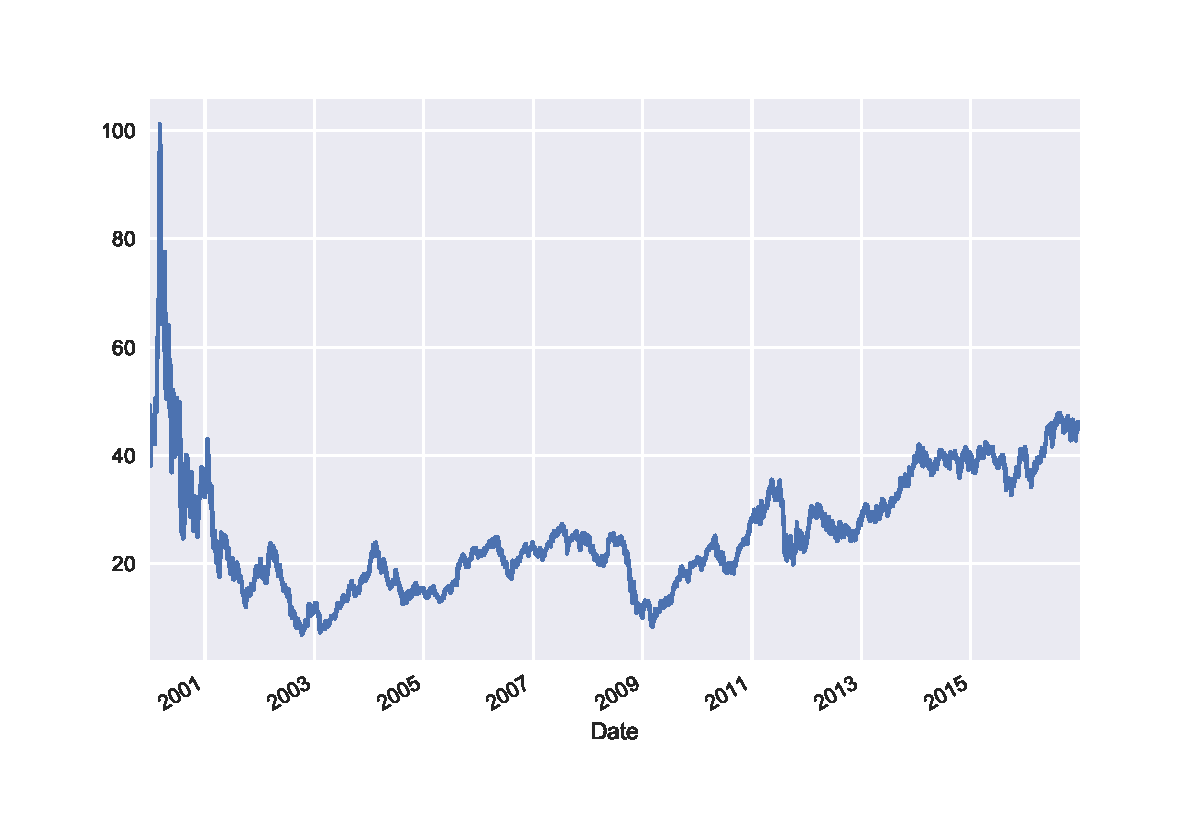
\includegraphics[width=\columnwidth]{src/stocks/simple/oneplot}\\
\captionof{figure}{Basic plot}
\label{fig:stock_oneplot}}
{\centering
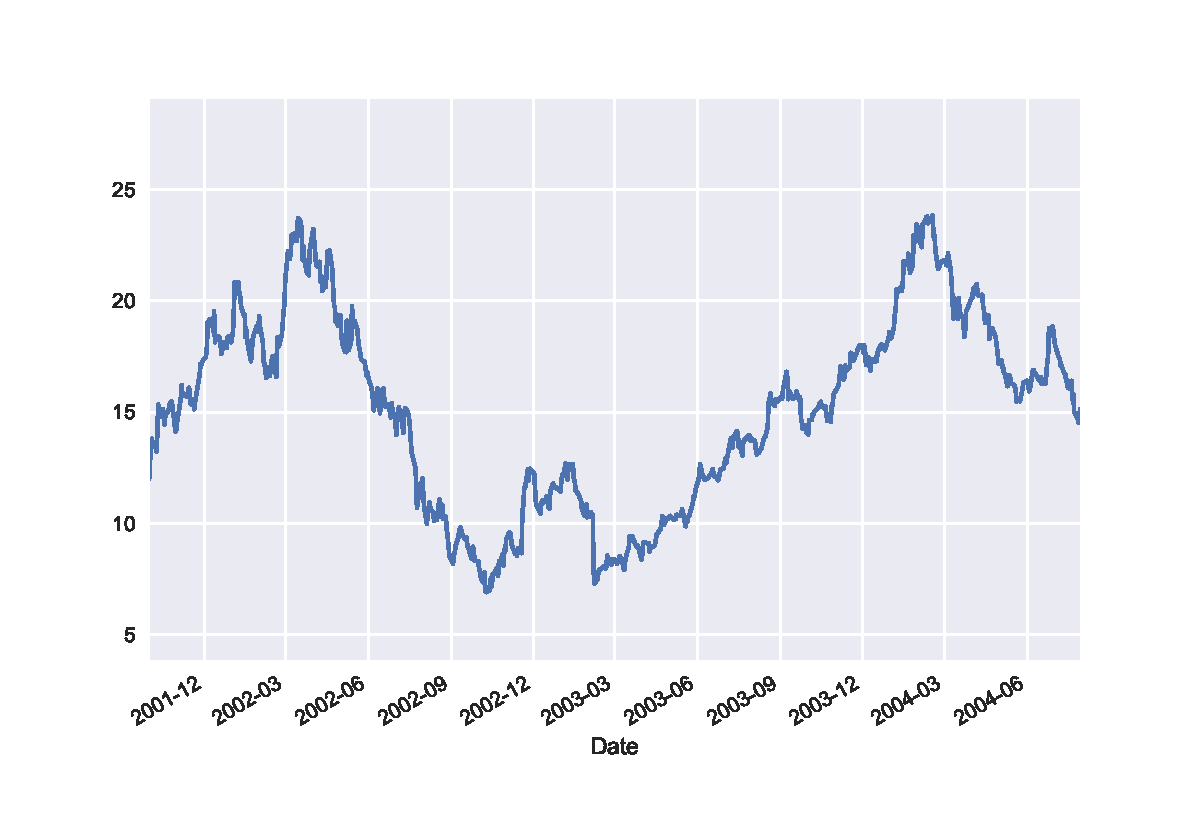
\includegraphics[width=\columnwidth]{src/stocks/simple/oneplot_zoom}\\
\captionof{figure}{Basic plot - zoomed}
\label{fig:stock_oneplot_zoom}}
\end{multicols}

\subsubsection{Moving average plot}

\bgroup
  \inputminted[linenos, breaklines=true, fontsize=\scriptsize, firstnumber=last]{python}{src/stocks/simple/3_moving_avg.py}
  \captionof{listing}{Moving average plot}
  \label{listing:ssimp_3}
\egroup

\begin{figure}[H]
    \centering
    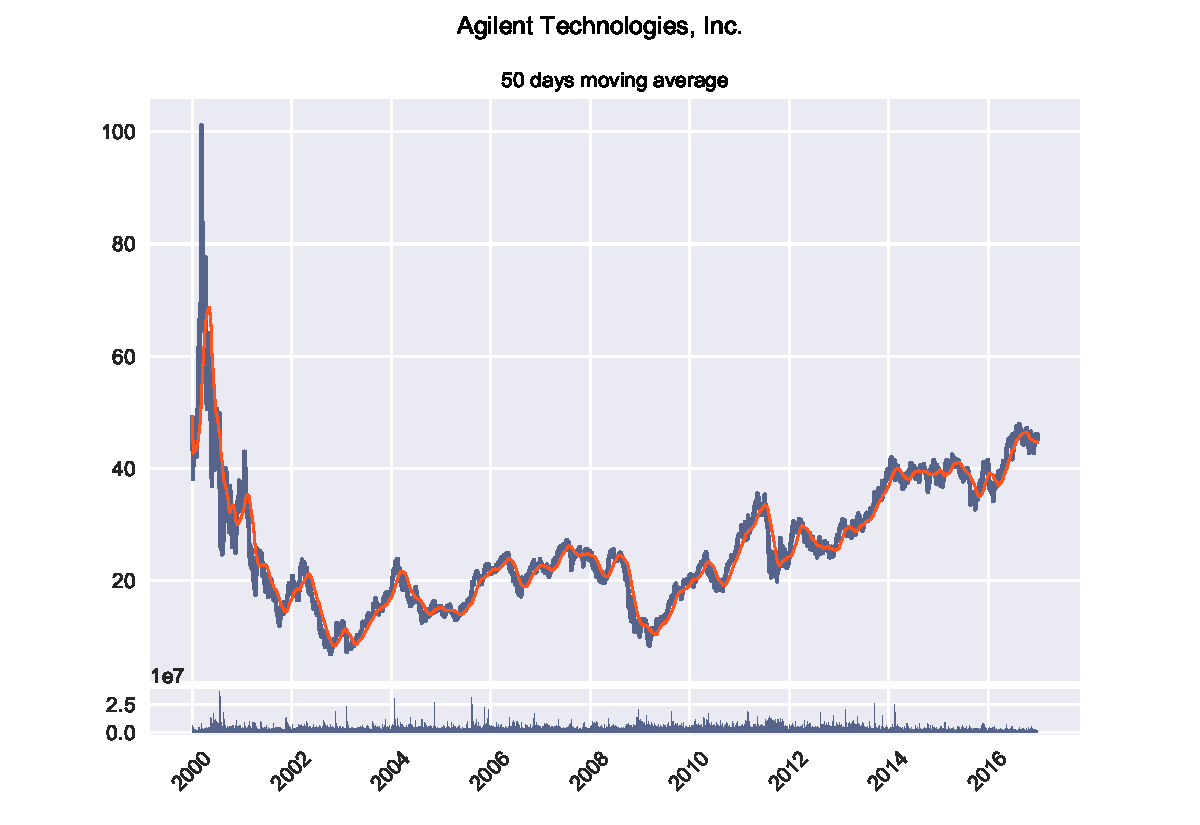
\includegraphics[width=\textwidth]{src/stocks/simple/movingavg}
    \caption{Moving average plot}
    \label{fig:stock_movingavg}
\end{figure}

\begin{figure}[H]
    \centering
    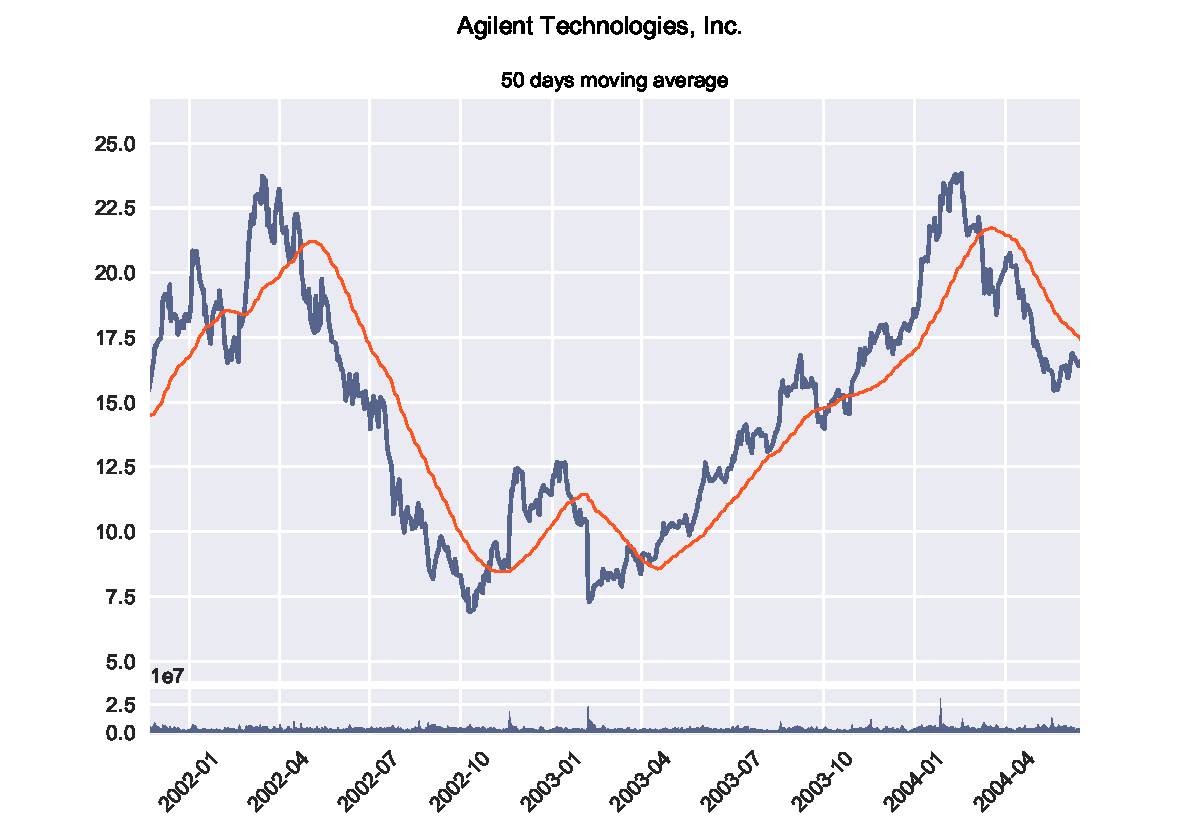
\includegraphics[width=\textwidth]{src/stocks/simple/movingavg_zoom}
    \caption{Moving average plot - zoomed}
    \label{fig:stock_movingavg_zoom}
\end{figure}

\subsubsection{Candlestick plot}

A candlestick plot is a way to visualize aggregated stock data that has originated in Japan and was popularized in the west by Steve Nison \cite{candlestick}. It employs a structure that is similar to box plots to show the stock’s opening, close, high and low prices for a specific time period - usually a day or a week. Usually, a entry for one day (or week, month, etc.) consists of the following: (1) a box, showing opening and close prices and (2) lines, or “shadows”, that show the high and low prices (you can see those on figure \ref{fig:stock_candlestick_zoom}). This, in combination with changing the color of the box to show whether the stock has gone up or down in price to create this plotting technique. Candlestick plotting is also often combined with a volume plot that shows how much trading was done in that time period (on the bottom in the example).

\begin{figure}[H]
    \centering
    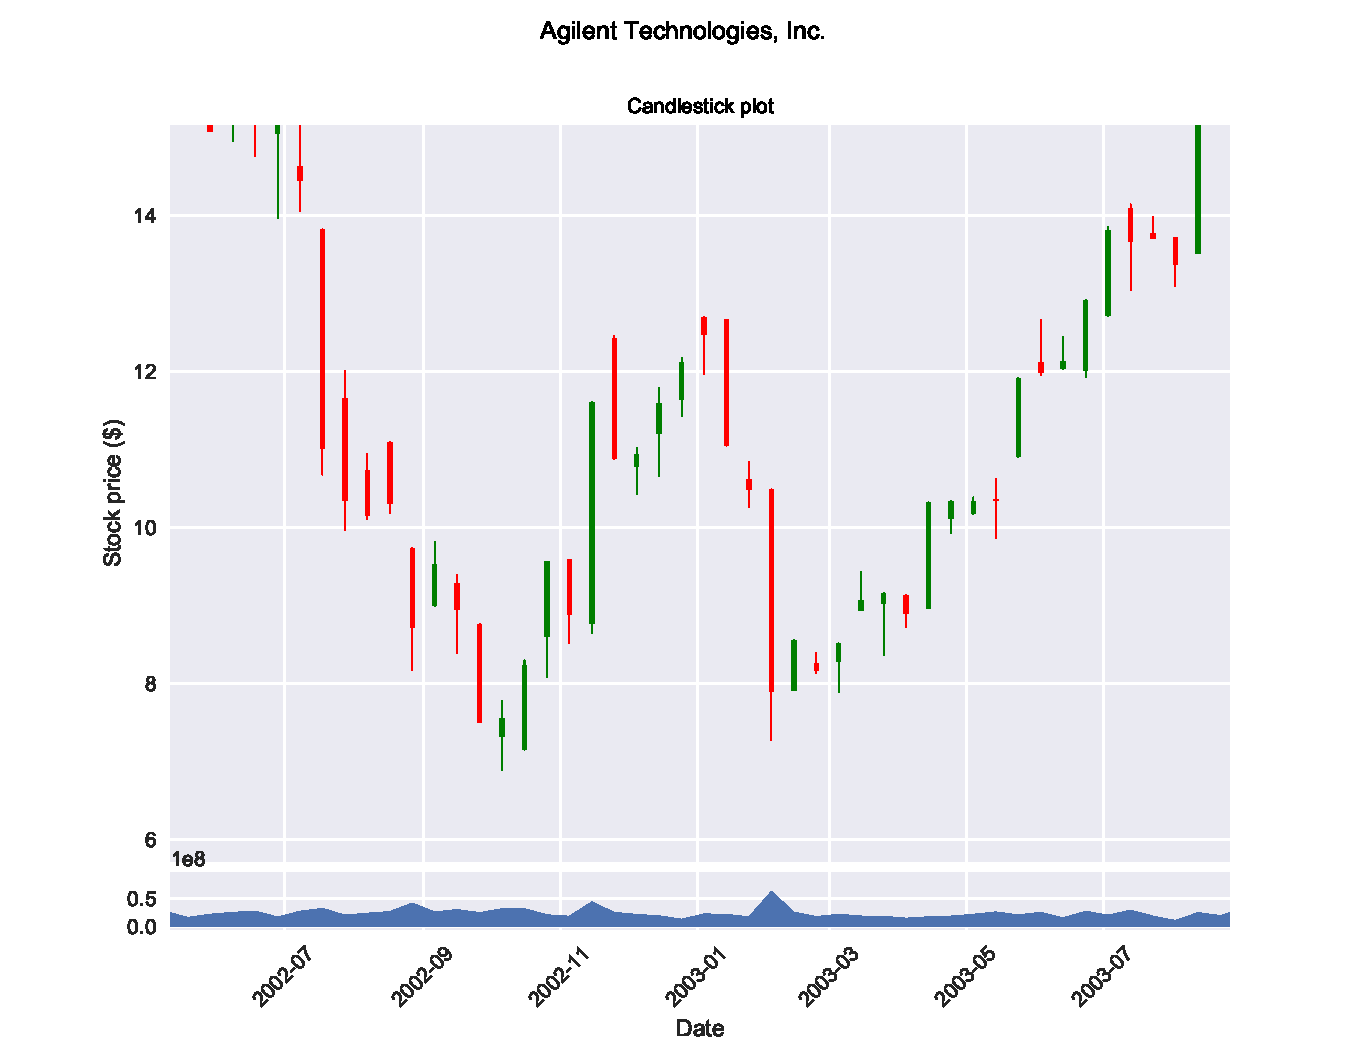
\includegraphics[width=\textwidth]{src/stocks/simple/candlestick_zoom}
    \caption{Candlestick plot - zoomed}
    \label{fig:stock_candlestick_zoom}
\end{figure}

The pandas package has some support for the candlestick plots, which, as you can see in the listing \ref{listing:ssimp_4_candle}, can be very useful when trying to create such plots by yourself.  You can use functions like \texttt{df[column].resample('time\_period')} to resample your data and then pair it with \texttt{df.ohlc()} to extract the open/high/low/close values from that aggregation. This, paired with \texttt{candlestick\_ohlc} function from \texttt{matplotlib.finance} module allows you to create candlestick plots rather quickly.

\bgroup
  \inputminted[linenos, breaklines=true, fontsize=\scriptsize, firstnumber=last]{python}{src/stocks/simple/4_candlestick.py}
  \captionof{listing}{Candlestick chart}
  \label{listing:ssimp_4_candle}
\egroup

As you can see in the figures \ref{fig:stock_candlestick_zoom} above and \ref{fig:stock_candlestick} below, the resulting plot is interactive and allows for the user to zoom in and only view the time period that they are interested in.

\begin{figure}[H]
    \centering
    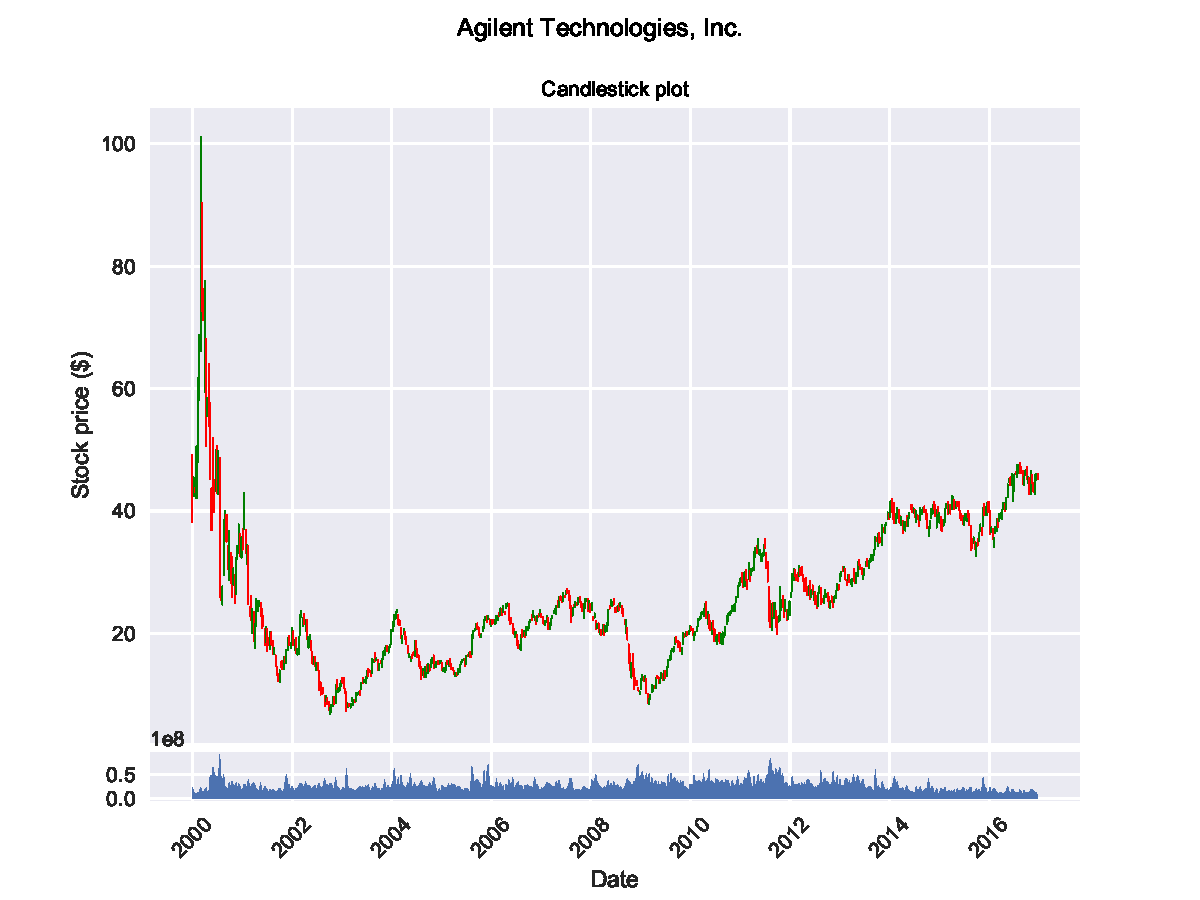
\includegraphics[width=\textwidth]{src/stocks/simple/candlestick}
    \caption{Candlestick plot}
    \label{fig:stock_candlestick}
\end{figure}


%-------------------------------------------------------------------------------
\newpage
\subsection{Stock correlation matrix visualization (matplotlib)} \label{ssec:stock_corr}
%-------------------------------------------------------------------------------

A correlation between two stock prices shows, whether a rise in price of one stock correlates with a rise or fall in price of another stock, or whether two stocks are completely independent.

A logical, albeit a bit inefficient, way to store correlation between a certain number of stocks is to create a so-called correlation matrix, whose structure you can see in table \ref{table:corr}.

Research like \cite{kwapien2006bulk} suggests that correlation matrix may contain useful information about the stock market, which makes it into a metric that can be used by stock investors that would like to diversify their investment portfolio as much as possible, thus ensuring that if one of the stocks they have invested in drops in price, the other ones remain stable.

\begin{table}[h!]
\centering
\caption{Correlation matrix structure}
\begin{tabular}{ | c | c | c | c | }
  \hline
  \ & Stock1 & Stock2 & Stock3 \\
  \hline
  Stock1 & 1 & corr(Stock1, Stock2) & corr(Stock1, Stock3) \\
  \hline
  Stock2 & corr(Stock2, Stock1) & 1 & corr(Stock2, Stock3) \\
  \hline
  Stock3 & corr(Stock3, Stock1) & corr(Stock3, Stock2) & 1 \\
  \hline
\end{tabular}
\label{table:corr}
\end{table}

Once we have this matrix, a question arises - how can we visualize it? In this example visualization, I'll use a heat map chart, because of how the correlation numbers can be treated as colors.

\bgroup
  \inputminted[linenos, breaklines=true, fontsize=\scriptsize]{python}{src/stocks/corr/1_get_data.py}
  \captionof{listing}{Reading the data into the memory}
  \label{listing:scorr_1}
\egroup


\bgroup
  \inputminted[linenos, breaklines=true, fontsize=\scriptsize, firstnumber=last]{python}{src/stocks/corr/2_problem_labels.py}
  \captionof{listing}{First attempt at making a correlation matrix}
  \label{listing:scorr_2}
\egroup

\bgroup
  \inputminted[linenos, breaklines=true, fontsize=\scriptsize, firstnumber=last]{python}{src/stocks/corr/3_fix.py}
  \captionof{listing}{Fixing the labelling}
  \label{listing:scorr_3}
\egroup

%-------------------------------------------------------------------------------
\newpage
\subsection{Predictive analysis with a LSTM neural network (keras)}
%-------------------------------------------------------------------------------



%===============================================================================
\newpage
\section{GRAPH DATA ANALYSIS}
%===============================================================================
%-------------------------------------------------------------------------------
\subsection{Project Overview}
%-------------------------------------------------------------------------------
\begin{easylist}
# Goals
## to show how to run community detection algorithms in igraph
## to show how to plot the communities using two different methods - datashader  (larger data) and cairo (smaller data)
## to show how to make the communities visually separable and how to incorporate node weights in the plot
# Tools(Libraries) used
## Why I chose igraph
\end{easylist}

\myparagraph{Packages needed}
\begin{easylist}
  # igraph
  # cairocffi
\end{easylist}

\cite{csardi2006igraph}

%-------------------------------------------------------------------------------
\newpage
\subsection{Preprocessing and igraph creation}
%-------------------------------------------------------------------------------
\begin{easylist}
# Importing the data form konekt
# Optimizing edges renaming with numpy vectorize/jit
\end{easylist}

Data source \cite{youtube_source}

%-------------------------------------------------------------------------------
\newpage
\subsection{Community detection (igraph)}
%-------------------------------------------------------------------------------

%-------------------------------------------------------------------------------
\newpage
\subsection{Plotting large graphs (datashader)}
%-------------------------------------------------------------------------------
%- - - - - - - - - - - - - - - - - - - - - - - - - - - - - - - - - - - - - - - -
\subsubsection{Simple plot}
%- - - - - - - - - - - - - - - - - - - - - - - - - - - - - - - - - - - - - - - -
\improvement[inline]{Add a note about how datashader failed to plot the entire graph and why it's not a good idea in the first place (hard to see the points)}
\myparagraph{Goals}

\begin{enumerate}
  \item To show how you can plot regular large graphs with datashader
  \item To show how you can plot large graphs while distinguishing communities in them
\end{enumerate}

\myparagraph{Description}


%- - - - - - - - - - - - - - - - - - - - - - - - - - - - - - - - - - - - - - - -
\subsubsection{Regular plot}
%- - - - - - - - - - - - - - - - - - - - - - - - - - - - - - - - - - - - - - - -

\myparagraph{Datashader introduction}

\myparagraph{Results}

\myparagraph{Results}

While datashader is certainly capable of plotting a huge amounts of data points, sometimes using that capability is a bad idea and only leads to dissappointing results.

\begin{figure}
    \centering
    
\includegraphics[width=\textwidth]{src/youtube/datashader/simple/fullgraph}
    \caption{Directly connected layout - Plot of the full graph}
    \label{fig:ds_fullgraph}
\end{figure}

%- - - - - - - - - - - - - - - - - - - - - - - - - - - - - - - - - - - - - - - -
\subsubsection{Plotting communities}
%- - - - - - - - - - - - - - - - - - - - - - - - - - - - - - - - - - - - - - - -



%-------------------------------------------------------------------------------
\newpage
\subsection{Plotting small graphs (igraph)}
%-------------------------------------------------------------------------------
%- - - - - - - - - - - - - - - - - - - - - - - - - - - - - - - - - - - - - - - -
\subsubsection{Goals and section overview}
%- - - - - - - - - - - - - - - - - - - - - - - - - - - - - - - - - - - - - - - -
\myparagraph{Goals}

\begin{enumerate}
  \item To show how to create a regular graph's plot, and consider the idea that its simplicity may make it harder to read
  \item To show how to create a graph plot with marked communities on it, and compare it to the regular plot in terms of ease of reading
  \item To show how to create a graph plot with marked communities that also shows the weight of its nodes, and compare this plot to the other two
\end{enumerate}

\myparagraph{Description}

In this section, I will show you how to plot a smaller (around 1000 nodes) portion of our graph using tools that are supported by igraph, in particular using its bindings to a C library called cairo. Since it is originally written in C and only provides an API that other languages can use, we will also have to use a package that will be able to connect python code to the C library itself. In this example, I'm using cairocffi as such package, hence the inclusion of \texttt{import cairocffi as cairo} in the starting import list. We have to import it as cairo, because otherwise igraph will attempt to use a different binding package, \texttt{pycairo}, which is quite outdated and can outright refuse to save vector images.

%- - - - - - - - - - - - - - - - - - - - - - - - - - - - - - - - - - - - - - - -
\subsubsection{Regular plot}
%- - - - - - - - - - - - - - - - - - - - - - - - - - - - - - - - - - - - - - - -
\myparagraph{Selecting vertices}

First thing that we have to do in this section is to select a subgraph for plotting. I have decided to settle on the subgraph of vertices with high degrees, because that meant that every node would be connected to many other nodes, and that can be a good example of how to deal with clutter on the plot.

In order to select this subgraph, you can use the \texttt{graph.vs.select(*args, **kwargs)} method in your graph. This method works differently based on what you pass it:\newline

\begin{enumerate}
  \item If you pass a list of integers into it \texttt{select([1,2,3])}, or skip the list and call \texttt{select(1,2,3)}, it will return vertices at those indexes
  \item If you pass a special keyword argument to it, it will select all nodes with a property that match that argument
  \item If you pass a function to it, it will call that function on every vertex and return all vertices that the function has returned \texttt{True} for
  \item If you don't pass anything into the function, it returns an empty list
\end{enumerate}

The select method has 8 special keyword arguments:
\begin{multicols}{2}
  \begin{itemize}
  \item \texttt{eq} - equal to
  \item \texttt{ne} - not equal to
  \item \texttt{lt} - less than
  \item \texttt{gt} - greater than
  \item \texttt{le} - less than or equal to
  \item \texttt{ge} - greater than or equal to
  \item \texttt{in} - value is in the given list
  \item \texttt{notin} - value is not in the given list
  \end{itemize}
\end{multicols}

Please note, that you have to include the name of your property before the special keyword: \texttt{graph.vs.select(age\_in=[19,20,21])}. You can see how I have used \texttt{gt} in the following example. The \texttt{\_degree} you see in front of it is a semi-private variable (since no variable is truly private in python) that keeps track of the degree of the vertex.

\bgroup
  \inputminted[linenos, breaklines=true, fontsize=\scriptsize]{python}{src/youtube/hdg/1_selecting.py}
  \captionof{listing}{Selecting nodes for the subgraph}
  \label{listing:iplot_1sel}
\egroup

\myparagraph{Styling the resulting plot}

There are many different options to choose from if you want to change how the graph appears on the screen. They are originally available as keyword arguments that you can pass to the \texttt{ig.plot()} function, but I advocate for putting all of them in a separate dictionary, since it takes away from the dissaray of having to include many options into one function call.

In this paper I will mainly focus on the layout option, as well as gloss over a couple of settings connected to the size of the vertices and edges, but if after reading this you will want to learn more about them, you can call \texttt{help(ig.plot)} while in a python interpreter to see the function's docstring.

One of the most important arguments provided to us is the layout one, since it changes how nodes and edges are positioned in the resulting plot. It is possible to choose from the following layouts\footnote{Visual comparison is available on the pages \pageref{fig:hdg_c1}-\pageref{fig:hdg_c9}}:

\begin{multicols}{2}
  \begin{itemize}
  \item Circle layout
  \item Star layout
  \item Grid layout
  \item Fruchterman Reingold layout \cite{yt_layout_fg}
  \item Fruchterman Reingold grid layout
  \item DrL layout \cite{yt_layout_dl}
  \item Graphopt layout \cite{yt_layout_graphopt}
  \item Kamada Kawai layout \cite{yt_layout_kk}
  \item Sugiyama layout \cite{yt_layout_sg}
  \item Random layout
  \item Large Graph layout
  \item Reingold Tilford layout (for trees) \cite{yt_layout_ft}
  \item Bipartite layour (for 2-layer graphs)
  \end{itemize}
\end{multicols}


As you can see in the listing, other options are responsible for things like edge width, vertex size and shape, where to save the file, et cetera.

The \texttt{bbox} argument is responsible for how big your final plot is going to be (in another words, it is declaring a limiting box on a figure that no vertex can cross).

The \texttt{target} keyword argument is also very useful - it specifies the name of the file that your final chart will be stored in, and supports multiple file extentions (PDF, SVG, PNG).  In the next section I will also explain you how to add a color palette to the dictionary in order to distinguish the communities that we will detect.

\bgroup
  \inputminted[linenos, breaklines=true, fontsize=\scriptsize, firstnumber=last]{python}{src/youtube/hdg/2_style_dict.py}
  \captionof{listing}{Creating a style dictionary}
  \label{listing:iplot_2sd}
\egroup

\myparagraph{Plotting and saving the resulting plot to a file}

\bgroup
  \inputminted[linenos, breaklines=true, fontsize=\scriptsize, firstnumber=last]{python}{src/youtube/hdg/3_plotting.py}
  \captionof{listing}{Plotting the image}
  \label{listing:iplot_3im}
\egroup

Since we have already constructed the keyword argument dictionary for the plot function, the rest becomes very clean and easy - we just have to pass the dictionary to the function while remembering to unroll it to convert it to key-value pairs.

\myparagraph{Layout comparison and revision of the results}

All of the plots generated in this section use the aforementioned style dictionary, while only changing the \texttt{['layout']} part of it.

\begin{multicols}{2}
{\centering

\includegraphics[width=\columnwidth]{src/youtube/hdg/comp/1_plot_crc}\\
\captionof{figure}{Circular layout}
\label{fig:hdg_c1}}
{\centering

\includegraphics[width=\columnwidth]{src/youtube/hdg/comp/2_plot_str}\\
\captionof{figure}{Star layout}
\label{fig:hdg_c2}}
\end{multicols}

Circular layout puts all vertices on a circle and then draws the edges between them, while the star layout puts one of the vertices in the middle an tries to center the plot around it. As you can see from the above figures, in this case they are almost non-distinguishable, and don't show any insights about the graph.

\begin{multicols}{2}
{\centering
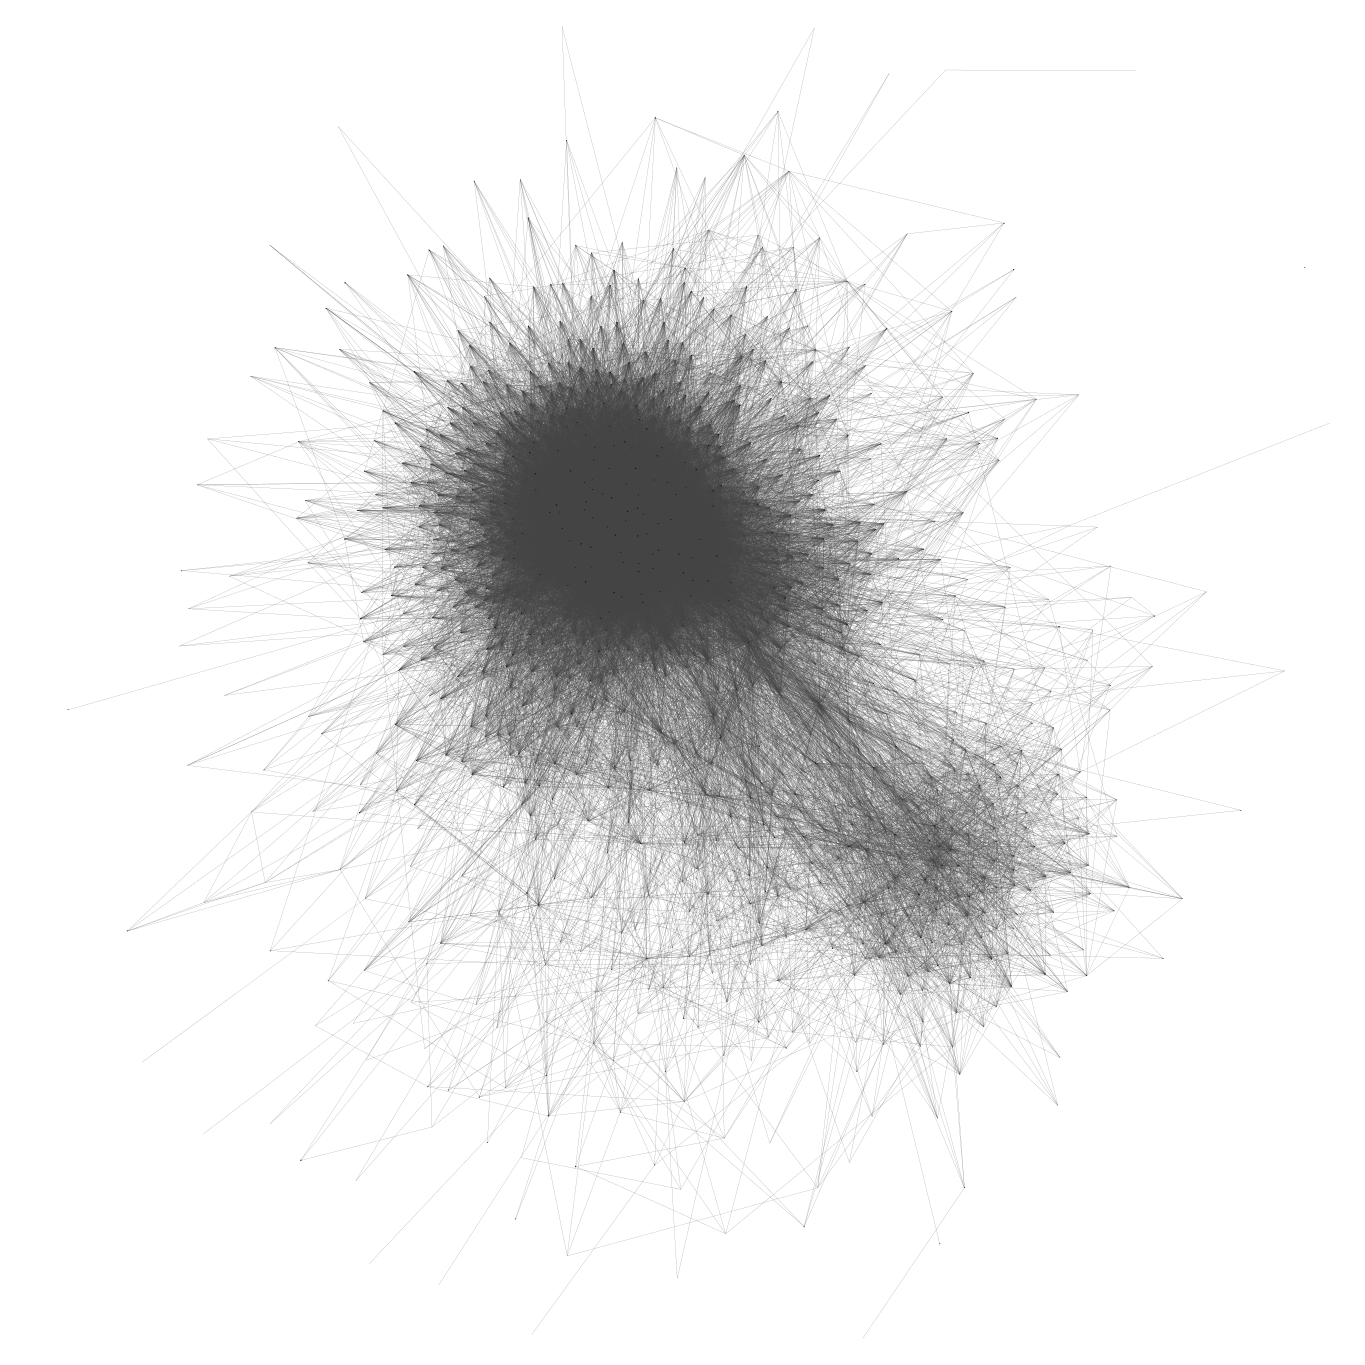
\includegraphics[width=\columnwidth]{src/youtube/hdg/hdg_simple}
\captionof{figure}{Fruchterman Reingold layout}
\label{fig:hdg_simple}}
{\centering
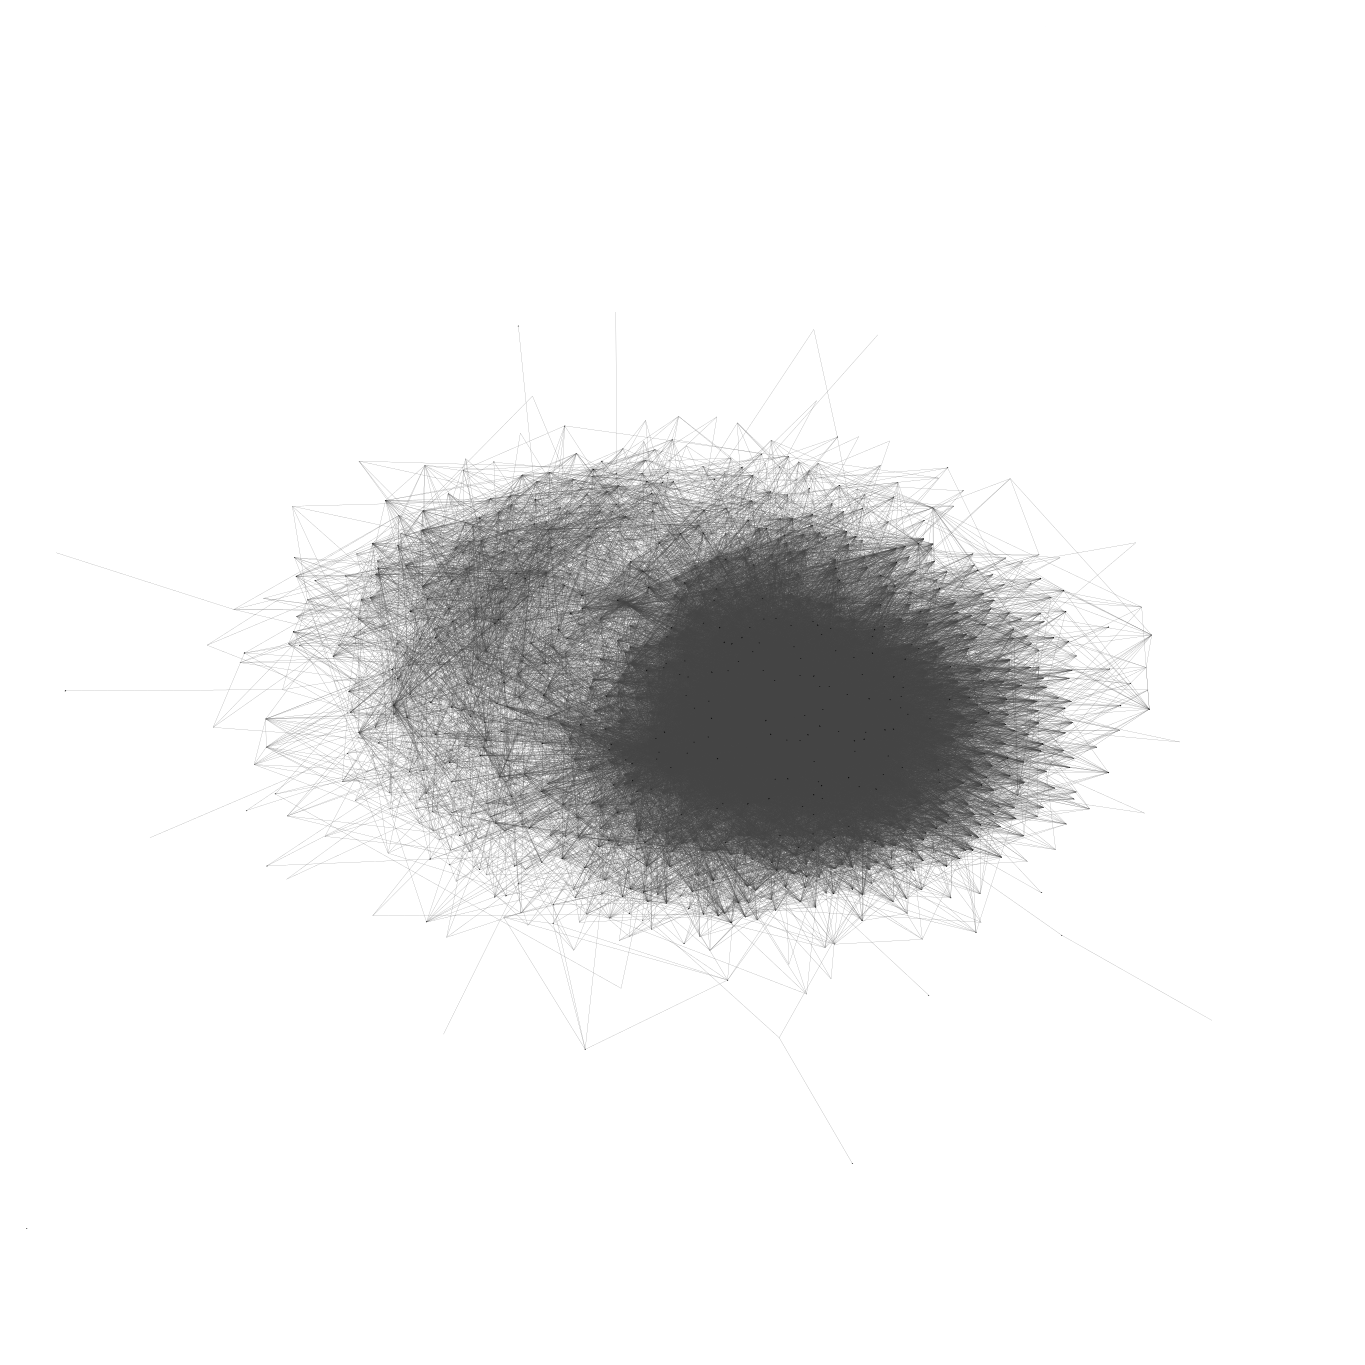
\includegraphics[width=\columnwidth]{src/youtube/hdg/comp/5_plot_kk}\\
\captionof{figure}{Kamada Kawai layout}
\label{fig:hdg_c5}}
{\centering

\includegraphics[width=\columnwidth]{src/youtube/hdg/comp/7_plot_drl}\\
\captionof{figure}{DrL layout}
\label{fig:hdg_c7}}
{\centering
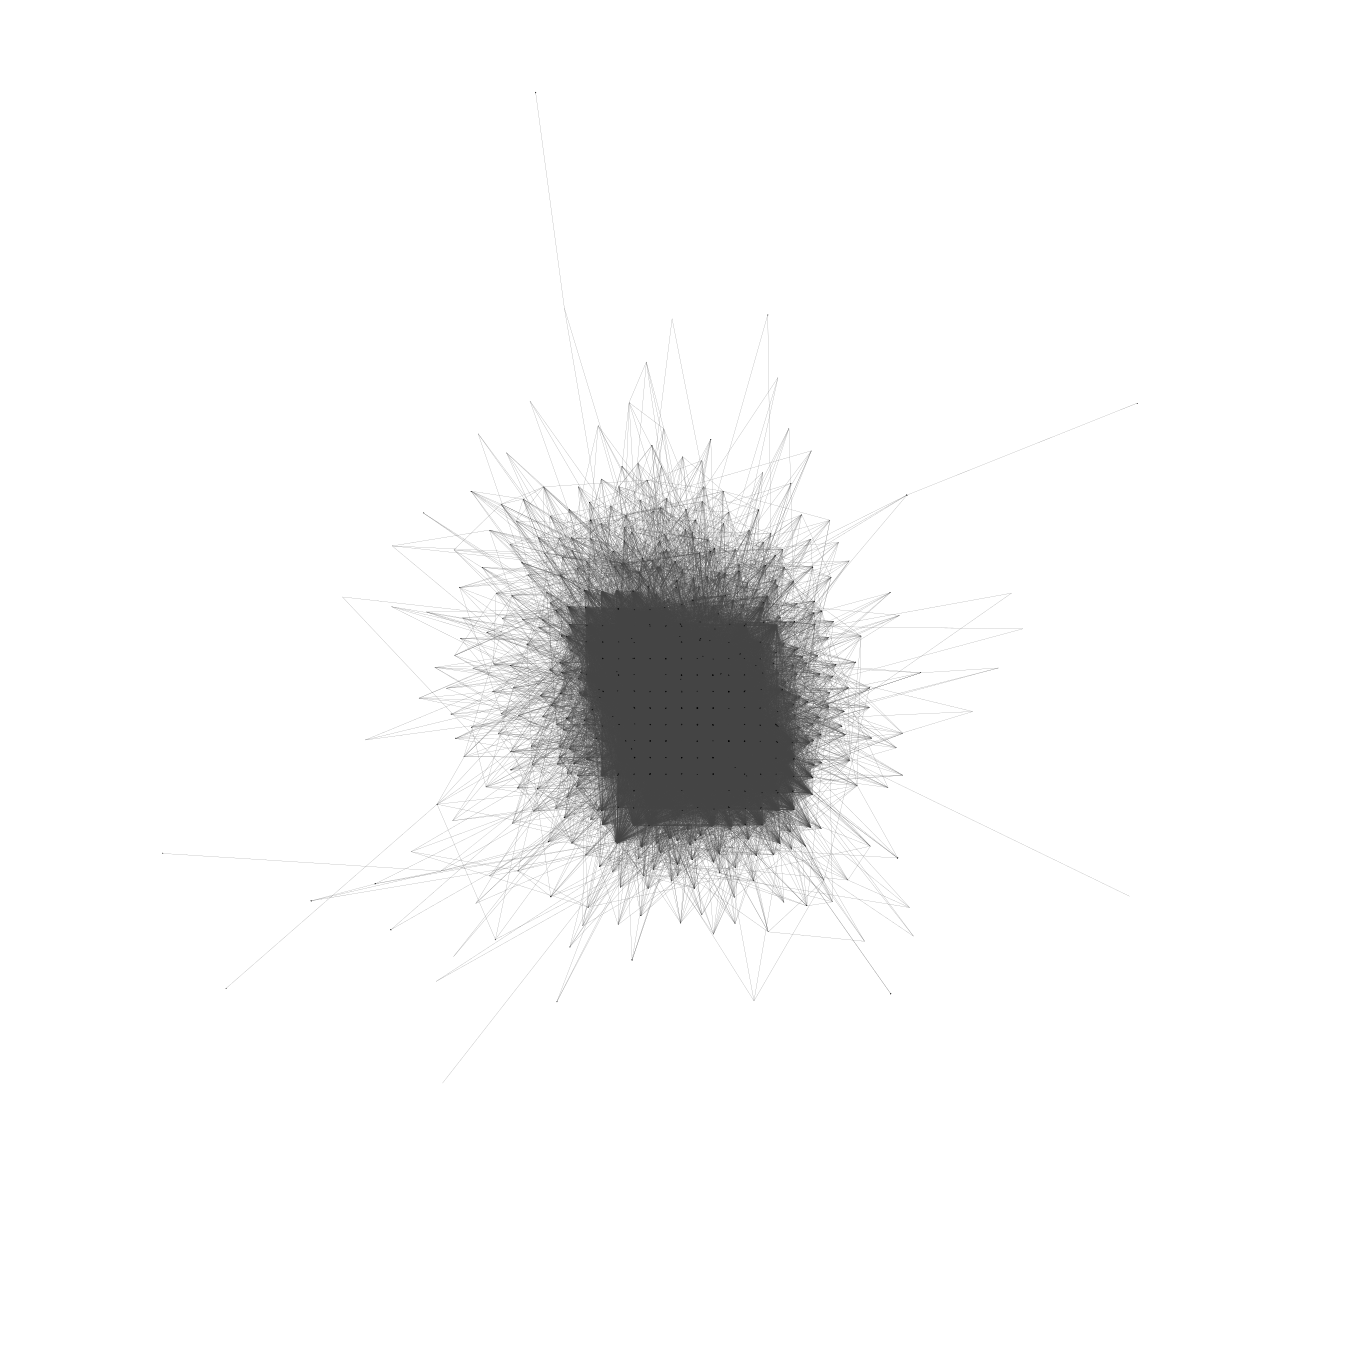
\includegraphics[width=\columnwidth]{src/youtube/hdg/comp/6_plot_ghopt}\\
\captionof{figure}{Graphopt layout}
\label{fig:hdg_c6}}
\end{multicols}

Force-directed algorithms like Fruchterman Reingold, Kamada Kawai, Graphopt and DrL  all use physics simulations to generate a plot. In this case, it led to Kamada Kawai and Graphopt making a plot that is mostly centered around one point, while Fruchterman Reingold and DrL layouts drew the graph by using two centers, thus highlighting two major communities within it. Unfortunately, DrL layout also spread the vertices too far away from each other, making the whole plot seem like a regular line.

Grid layouts put the vertices on an imaginary mesh, and then draw the connections between them. They can be useful for smaller graphs, but as you can see from the figures below, one can hardly infer any information from these if the amount of points is large enough.

\begin{multicols}{2}
  {\centering
  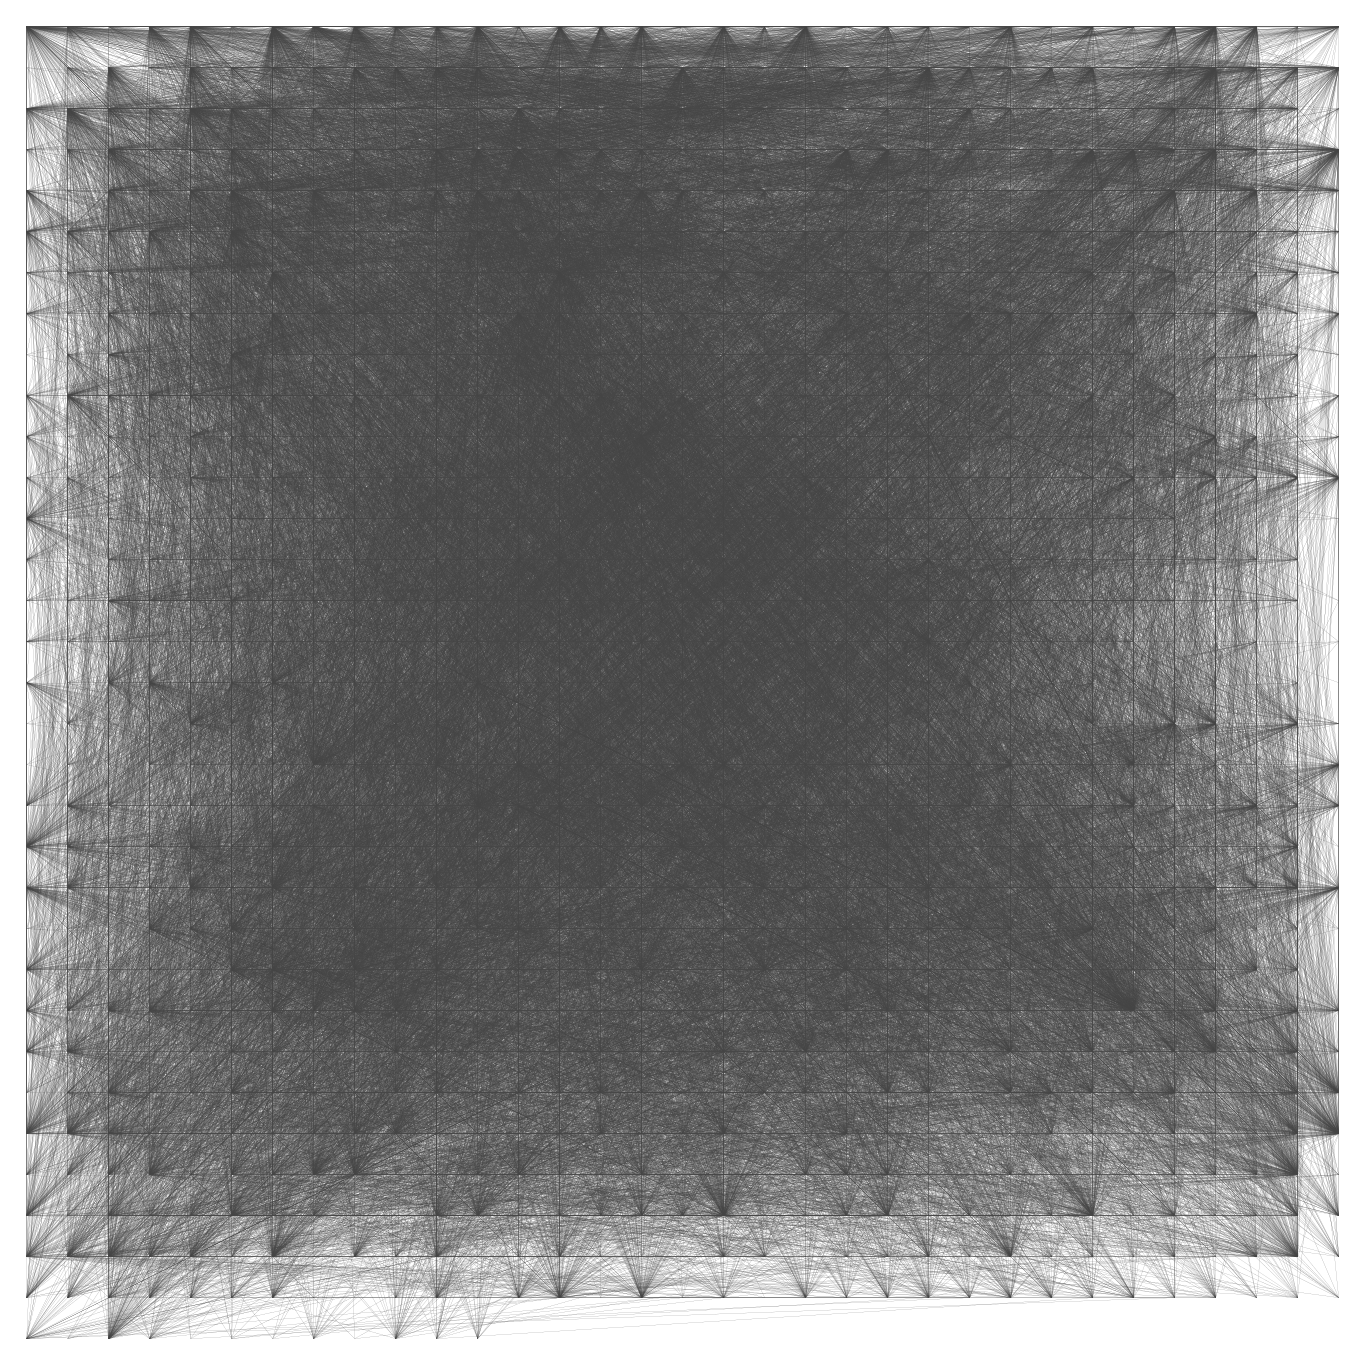
\includegraphics[width=\columnwidth]{src/youtube/hdg/comp/3_plot_grd}\\
  \captionof{figure}{Grid layout}
  \label{fig:hdg_c3}}
  {\centering
  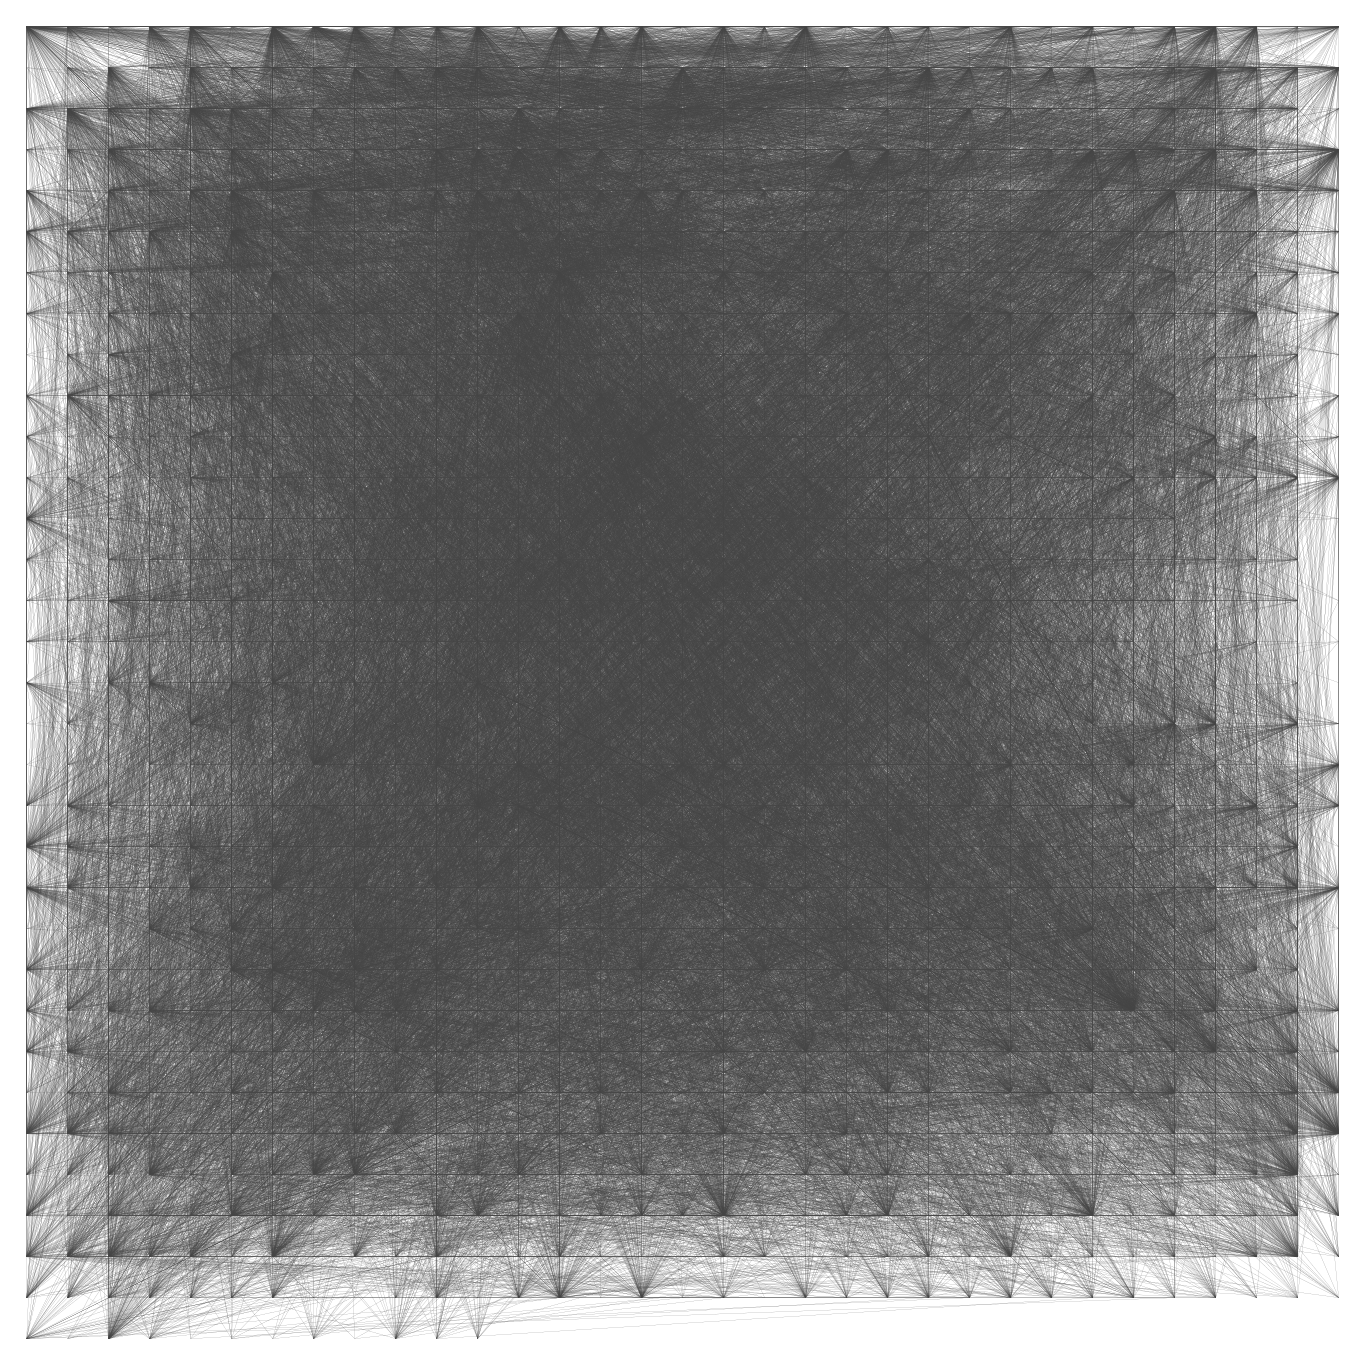
\includegraphics[width=\columnwidth]{src/youtube/hdg/comp/4_plot_frgrid}\\
  \captionof{figure}{Fruchterman Reingold grid layout}
  \label{fig:hdg_c4}}
\end{multicols}

Random layout, as its name suggests, places vertices on random points in the plot and then proceeds to draw the edges between them. Sugiyama layout tries to put vertices on different rows of the plot while directing their edges downwards, and is most suited for trees and not a social network graph like the one in this example.

\begin{multicols}{2}
  {\centering
  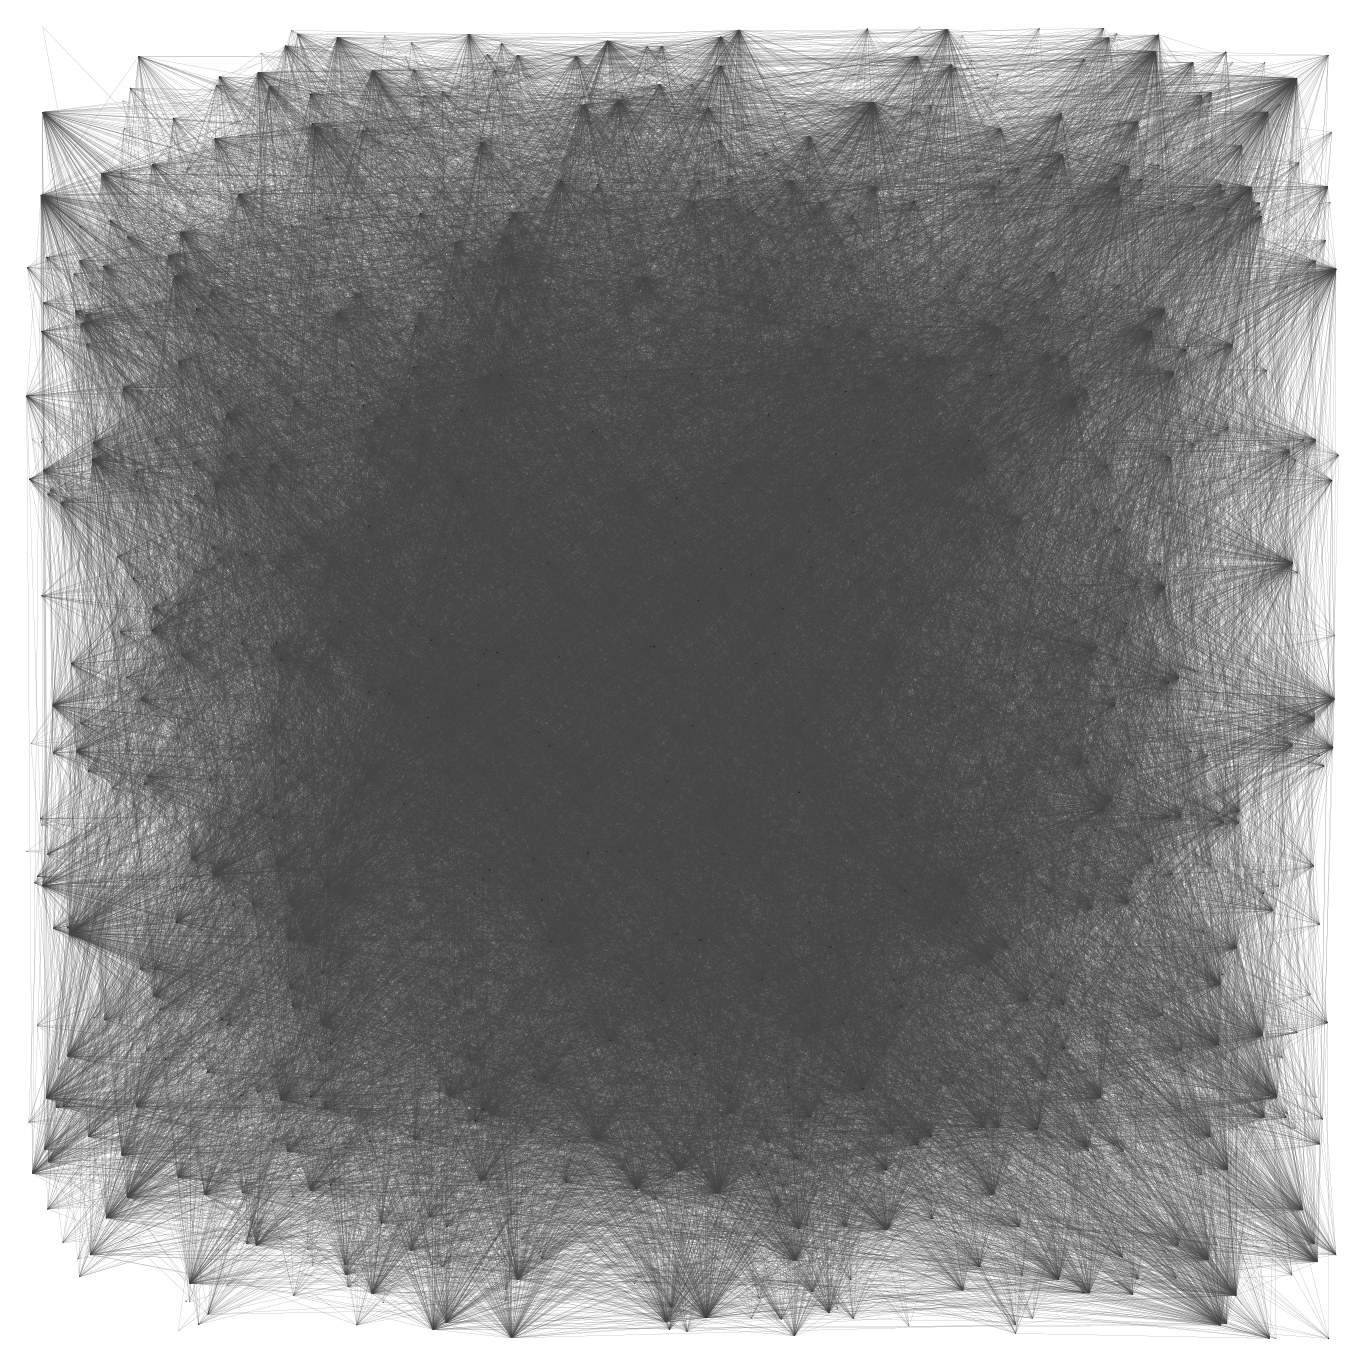
\includegraphics[width=\columnwidth]{src/youtube/hdg/comp/8_plot_random}\\
  \captionof{figure}{Random layout}
  \label{fig:hdg_c8}}
  {\centering
  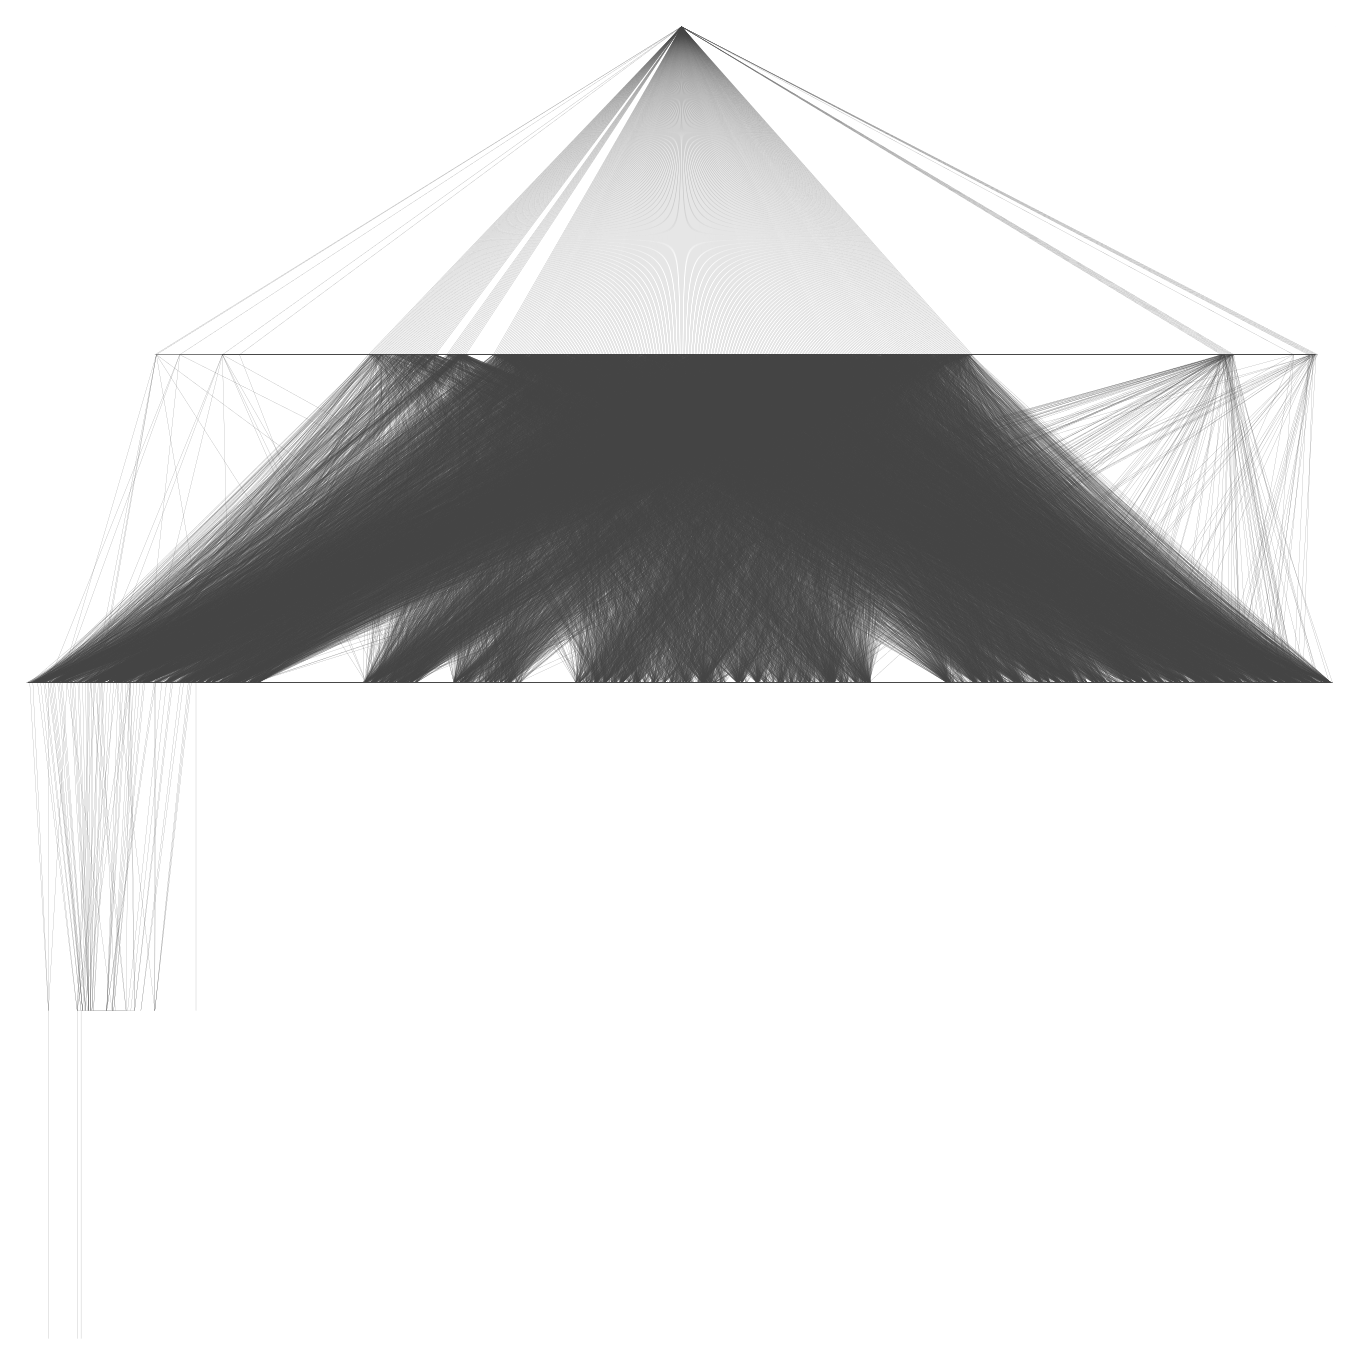
\includegraphics[width=\columnwidth]{src/youtube/hdg/comp/9_plot_sgy}
  \captionof{figure}{Sugiyama layout}
  \label{fig:hdg_c9}}
\end{multicols}

While igraph makes it quite easy to make regular plots like these, they don't provide one with much insight into the data itself. Even though you could look at the picture made using the Fruchterman Reingold layout, and detect two major communities in the network with a naked eye, other layouts aren't as simple to read. Still, I find that force-directed layouts like Fruchterman Reingold represented the social network graph better than other layouts.

%- - - - - - - - - - - - - - - - - - - - - - - - - - - - - - - - - - - - - - - -
\subsubsection{Community plot}
%- - - - - - - - - - - - - - - - - - - - - - - - - - - - - - - - - - - - - - - -
\myparagraph{Clustering the subgraph}

The size of the subgraph we're clustering is smaller than the one used in the datashader example, so using infomap right away without needing to cluster it with the louvain algorithm in advance is reasonable. In here I'm also storing the node's membership list into a variable, because we will need it later to color edges.

\bgroup
  \inputminted[linenos, breaklines=true, fontsize=\scriptsize]{python}{src/youtube/hdg_com/1_clustering.py}
  \captionof{listing}{Using infomap to cluster the subgraph}
  \label{listing:iplot_1cl}
\egroup

\myparagraph{Making communities visible}

There are a couple of ways to make communities in your graph more visible on the resulting plot. You could (1) use color to distinguish between them, (2) draw vertices from one community close to each other, (3) separate communities by drawing their boundaries, or (4) label each vertice with their community label. Some of those techniques are only effective when applied to very small graphs (like labeling), while other are a better fit for a medium-sized graph like the one used in this example.

In this example, I have decided to color all vertices within a community and edges between them using one color and to assign very heavy weights to them, and used a more neutral color for edges between vertices that belong to two different communities as well as assigning a very light weight to them. This guarantees that when I will run the fruchterman reingold layout algorithm, the communities will be pulled apart from each other, while vertices in a community will remain together.

As for colors, since the number of communities changed whenever I ran the infomap algorithm, I have decided to go with a randomized approach and just generate a random color for each community using a list comprehension and the \texttt{random.randint(min, max)} function that would give me a color-representing number that then would be converted to hex using the \texttt{06x} string format.

\bgroup
  \inputminted[linenos, breaklines=true, fontsize=\scriptsize, firstnumber=last]{python}{src/youtube/hdg_com/2_initializing_colors.py}
  \captionof{listing}{Initializing color and weight lists}
  \label{listing:iplot_2ic}
\egroup
\ \\
To assign color to a vertice in igraph, you can just add an attribute \textquotedblleft color\textquotedblright to the vertex, and igraph with cairo will fill that vetice with that color if it is in the pallette that you have to assign in the keyword argument (or style) dictionary. The enumerate function adds an id to the every member of an iterable that you pass into it, so I used it to get access to the community ID numbers, since the \texttt{comm}  variable is just a list of vertices. Then I proceeded to iterate through every vertice and assign a matching color to them.\\

\bgroup
  \inputminted[linenos, breaklines=true, fontsize=\scriptsize, firstnumber=last]{python}{src/youtube/hdg_com/3_colors_looping_vert.py}
  \captionof{listing}{Assigning color to vertices}
  \label{listing:iplot_3cl}
\egroup
\ \\
I did a very similar thing to the edges, except this time I have checked whether both of their ends are in one community and assigned different color and weights based on that.

\bgroup
  \inputminted[linenos, breaklines=true, fontsize=\scriptsize, firstnumber=last]{python}{src/youtube/hdg_com/4_colors_looping_edge.py}
  \captionof{listing}{Assigning color to edges}
  \label{listing:iplot_3ce}
\egroup

\myparagraph{Styling the resulting plot}

In order for igraph to be able to use a color, it has to be in it's palette. You can either use standard colors from the standard palette or create your own PrecalculatedPallette, passing the color list into the function (color can be specified using hex, rgb or their english names like \textquotedblleft red\textquotedblright). So, while the edges' and vertices' colors are decided based on their color attribute, the palette that those colors will be drawn from have to be specified in the style dictionary or as a regular keyword argument. You can also use the \texttt{mark\_groups} option if you either don't want to color the vertices or edges yourself or just want to make sure that every group is clearly delineated and is very visible\footnote{You can see how it looks on the pages \pageref{fig:hdg_com}-\pageref{fig:hdg_com_marked}}.

One more new thing in this code listing is the \texttt{edge\_order\_by} argument, and it is quite important for this example, since it determines the order that the edges are drawn in. So, if we order them by weight that means that the the gray edges between communities that have lighter weights will be drawn first, and the heavier and more colorful edges inside of the communities will be drawn on top of them.

\bgroup
  \inputminted[linenos, breaklines=true, fontsize=\scriptsize, firstnumber=last]{python}{src/youtube/hdg_com/5_styling_prop.py}
  \captionof{listing}{Styling using graph properties}
  \label{listing:iplot_5sg}
\egroup

\bgroup
  \inputminted[linenos, breaklines=true, fontsize=\scriptsize, firstnumber=last]{python}{src/youtube/hdg_com/6_style_dict.py}
  \captionof{listing}{Styling using a style dict}
  \label{listing:iplot_6sd}
\egroup

\myparagraph{Plotting and reviewing the results}

As you can see from the listing below, the plotting code didn't change from the last section, because all variable arguments have been placed in the style dictionary.

\bgroup
  \inputminted[linenos, breaklines=true, fontsize=\scriptsize, firstnumber=last]{python}{src/youtube/hdg_com/7_plotting.py}
  \captionof{listing}{Saving the plot to a file}
  \label{listing:iplot_7sv}
\egroup

\begin{figure}[ht]
    \centering
    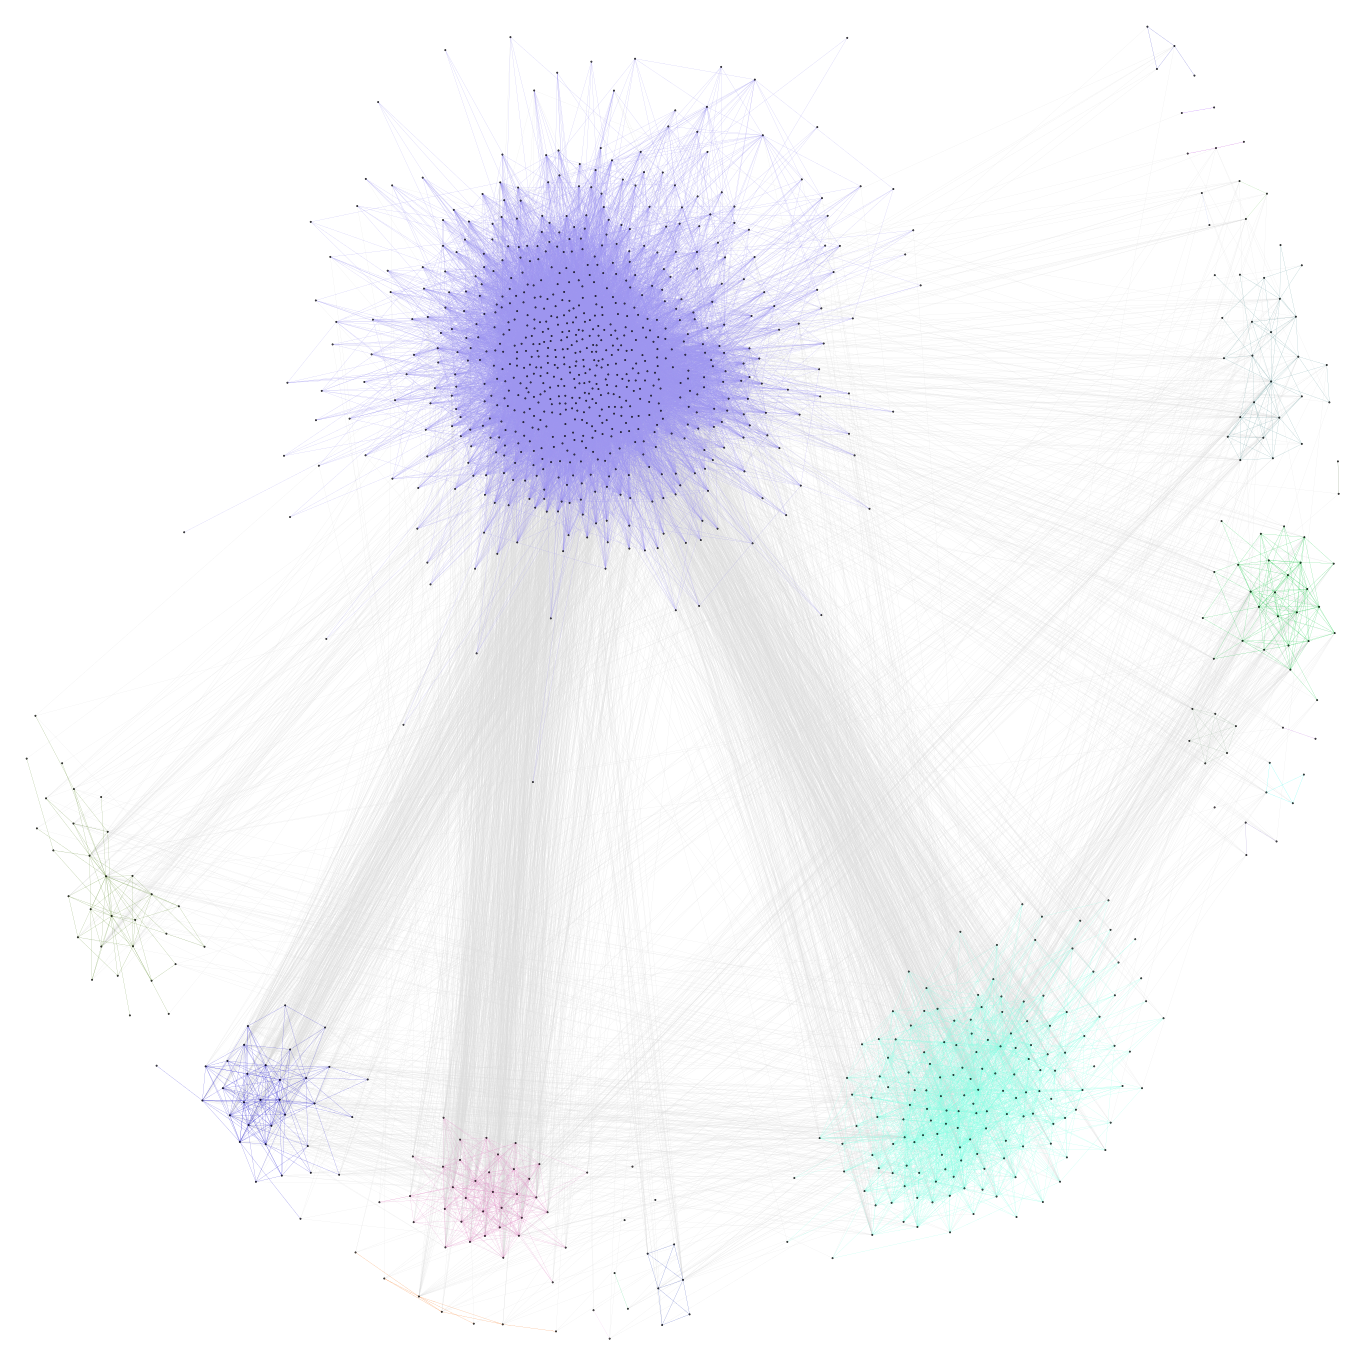
\includegraphics[width=\textwidth]{src/youtube/hdg_com/hdg_com}
    \caption{Community plot - Fruchterman Reingold layout}
    \label{fig:hdg_com}
\end{figure}

Looking at this plot, I find that the clear separation between groups and their coloring makes them easier to distinguish from each other, even if the groups could be made more prominent by changing their colors or increasing the edge thickness.

\begin{figure}[H]
    \centering
    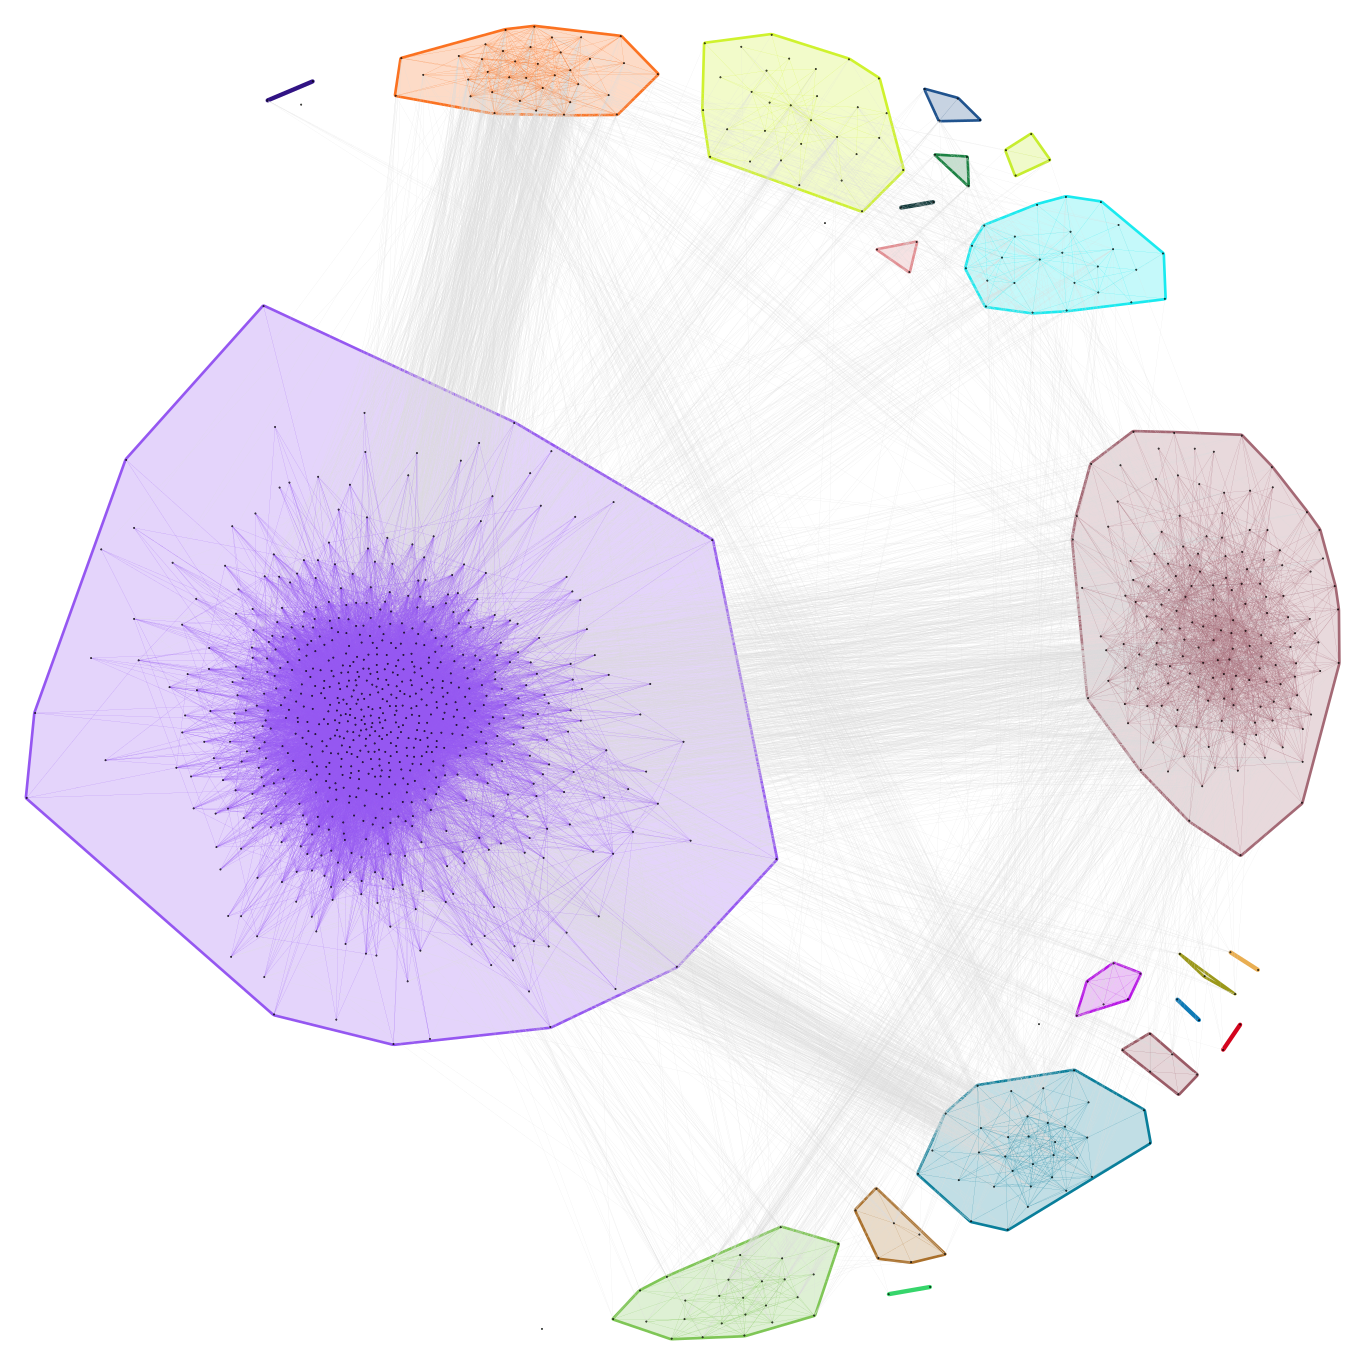
\includegraphics[width=\textwidth]{src/youtube/hdg_com/hdg_com_marked}
    \caption{Community plot - delineated groups - Fruchterman Reingold layout}
    \label{fig:hdg_com_marked}
\end{figure}

The delineated plot separates the communities even more than the regular coloring does, and adds boundaries that make even smallest groups of 2-3 vertices visible due to the bold lines connecting them. The problem with this plot is that the boundaries that separate the groups are drawn first, which makes them being crossed over by the edges that connect different communities. While that could be changed, the way of doing that would have to be very roundabout due to the delineation itself being just a true or false check in the plot function. I think that it may have been done intentially, just so you could actually see the edges properly.

To sum up, adding some kind of order with the groups and colors is, in my mind, a major improvement compared to the plots that were generated in the last section.

%- - - - - - - - - - - - - - - - - - - - - - - - - - - - - - - - - - - - - - - -
\subsubsection{Weighted community plot}
%- - - - - - - - - - - - - - - - - - - - - - - - - - - - - - - - - - - - - - - -
\myparagraph{Pagerank application}

Pagerank\cite{pagerank} is an algorithm developed by, among others, Larry Page and Sergey Brin that was used as a basis for the Google search engine. It uses a number of links to a specific vertex (originally, a webpage) to evaluate their importance. This metric is used as the weight of the vertices in this example. The pagerank implementation in the igraph package already auto assigns the weight, so you don't have to do that yourself.


\bgroup
  \inputminted[linenos, breaklines=true, fontsize=\scriptsize]{python}{src/youtube/hdg_weighted/1_pagerank.py}
  \captionof{listing}{Using pagerank to assign weights to vertices}
  \label{listing:iplot_1pg}
\egroup

\myparagraph{Style dictionary}

Style dictionary for the weighted graph is very similar to the one that was used to create the community plot, with an additions of weights as a keyword argument to pass to the fruchterman reingold layout and vertice size now depending on it's weight instead of being constant. As you can see from the code listing, the \texttt{vertex\_size} requires either a constant number or a iterable of all vertices' weights.

\bgroup
  \inputminted[linenos, breaklines=true, fontsize=\scriptsize, firstnumber=last]{python}{src/youtube/hdg_weighted/2_style_dict.py}
  \captionof{listing}{Styling using a style dict}
  \label{listing:iplot_32sd}
\egroup

%
\myparagraph{Plotting and reviewing results}

The plot function call in this case is the same as in two previous ones - \texttt{ig.plot(hdg\_subgraph, **hdg\_style)}.

Comparing this plot to the previous two, this one clearly presents the most information out of the three. If in the first section we had to only deal with the vertices and edges themselves, now we not only have communities of vertices that should be grouped, we also have different sizes of vertices inside those communities. While pagerank is an algorithm that always values nodes with more connection higher, thus making the violet community the most prominent group, if this chart was made using a different data set it could reveal something like the least populated community being the most important or something among those lines.

\begin{figure}
    \centering
    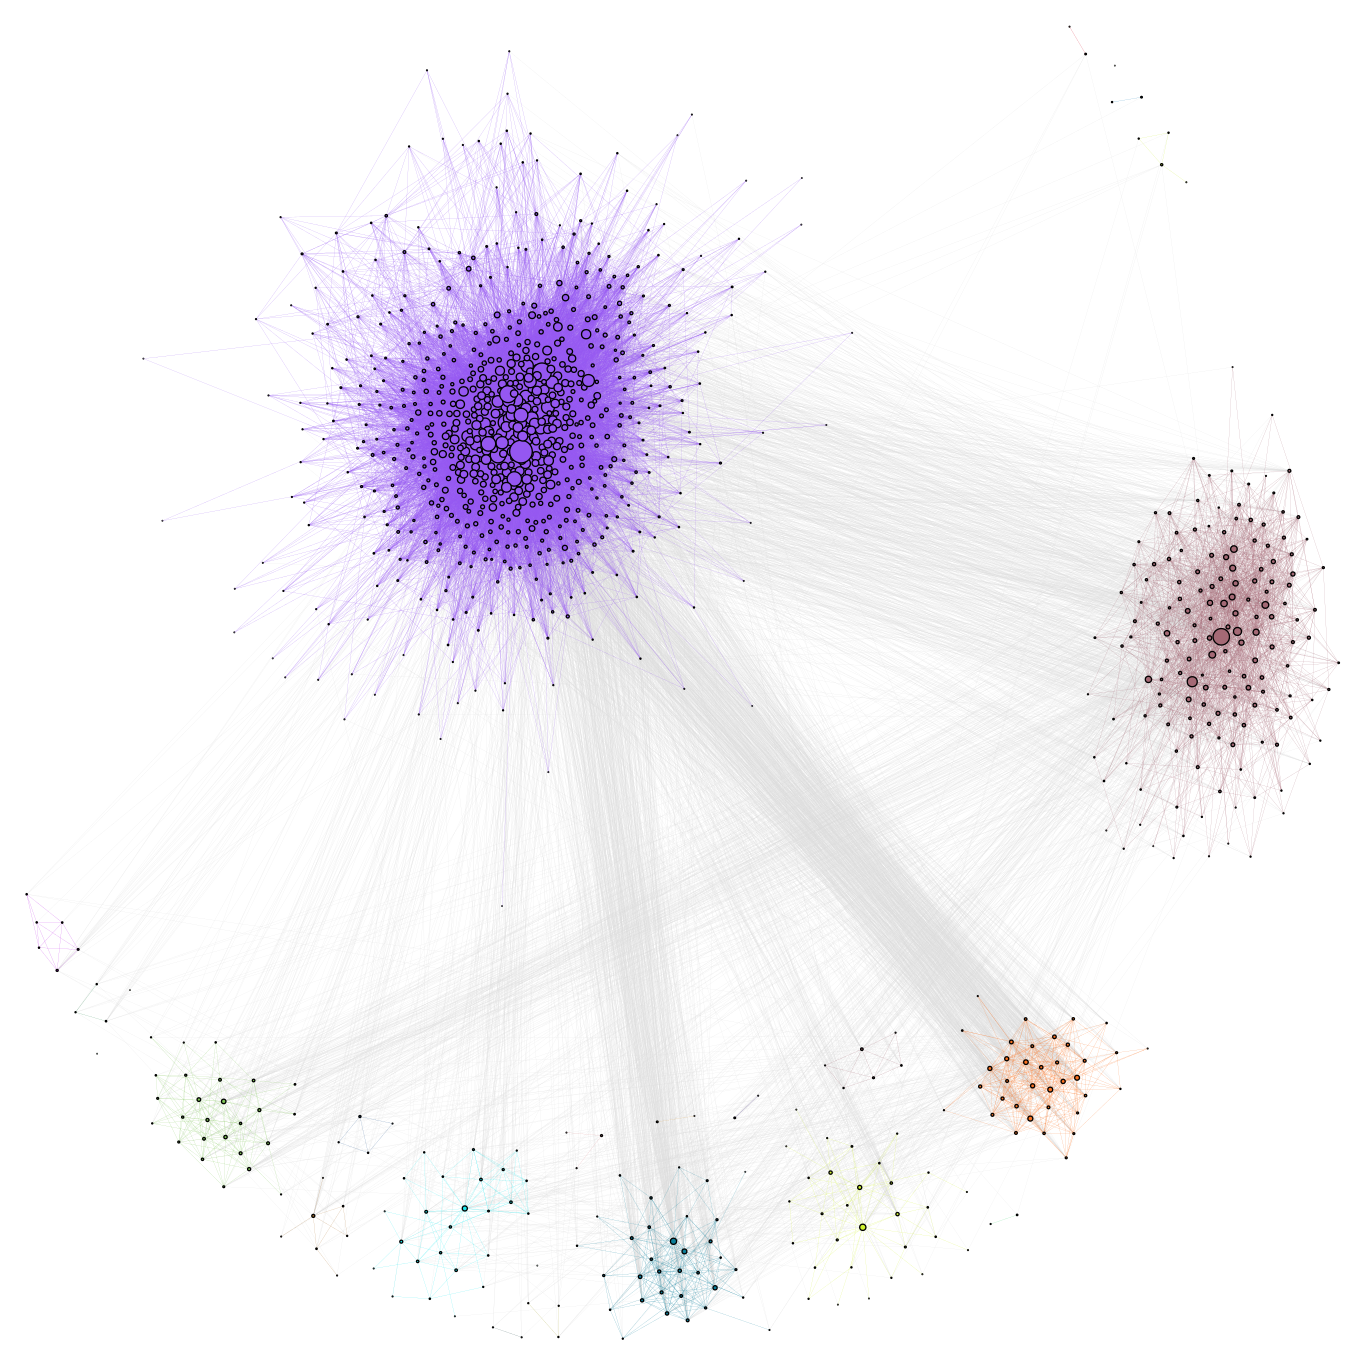
\includegraphics[width=\textwidth]{src/youtube/hdg_weighted/hdg_pg_fg}
    \caption{Weighted plot - Fruchterman Reingold layout}
    \label{fig:hdg_pg_fg}
\end{figure}


%===============================================================================
\newpage
\section{GEODATA ANALYSIS}
%===============================================================================

%-------------------------------------------------------------------------------
\subsection{Project Overview}
%-------------------------------------------------------------------------------
\begin{easylist}
# Goals
## to show how to deal with geodata in python
# Plots
## KPI per country (Basemap)
 ## Plot - Chikago Taxi (datashader)
\end{easylist}


%===============================================================================
\newpage
\section{CONCLUSION}
%===============================================================================

Include data types that we omit - biological data, food data, describe what you'd like for others to research.

% Literature references
\newpage

\printbibliography[heading=bibnumbered, title={REFERENCES}]

\end{document}
